\documentclass[11pt]{article}
\usepackage[margin=1in]{geometry}
\usepackage[T1]{fontenc}
\usepackage{lmodern}
\usepackage{amsmath,amssymb}
\usepackage{graphicx}
\usepackage{booktabs}
\usepackage{placeins}
\usepackage{algorithm}
\usepackage{algpseudocode}
\usepackage{listings}
\lstset{basicstyle=\ttfamily\scriptsize, columns=fullflexible, keepspaces=true, frame=tb,
  captionpos=b, showstringspaces=false, breaklines=true, breakatwhitespace=true, aboveskip=8pt, belowskip=4pt}
\usepackage[numbers,sort&compress]{natbib}
\usepackage[hidelinks]{hyperref}

\newcommand{\pool}{\mathcal{E}}
\newcommand{\reach}{\mathcal{P}}
\newcommand{\res}{\mathcal{R}}
\newcommand{\hot}{\mathcal{H}}
\newcommand{\topk}{\operatorname{top}_k}
\newcommand{\ci}[2]{[$#1$, $#2$]}
\newcommand{\repo}{https://github.com/jackmaxwil/keep}
\newcommand{\src}[1]{\href{\repo/blob/main/#1}{\nolinkurl{#1}}}

\title{Pruning Is a Frozen Cache:\\Unifying Pruning, Quantization and Offloading\\in Mixture-of-Experts Inference\thanks{Code: \url{https://github.com/jackmaxwil/keep}}}
\author{Jack Mazac}
\date{}

\begin{document}
\maketitle

\begin{abstract}
The most capable open language models do not fit on the computers people own. The one we
study holds 289\,GB of weights in its experts; an Apple M4 Max laptop has 128\,GB
of memory and even at 2 bits a weight the experts need 141\,GB. Its design leaves an
opening. It is a mixture of experts: each layer holds hundreds of small networks
and each token (roughly a word) uses only a few, so most weights sit idle. Three techniques
exploit this, each at a price: pruning deletes experts for good, quantization blurs them
into fewer bits, and offloading leaves them on storage and stalls to fetch one.

We treat the three as one decision: which bytes are in memory when a token arrives. A setup is
described by which experts may be selected (\emph{reach}), which are in memory
(\emph{residency}), how many bits each carries (\emph{precision}), and what happens when a
selected expert is absent. Seen this way, pruning is a frozen cache, a set in memory that never
changes. \emph{Routed residency} lets it change: every expert stays reachable on storage, a
missing one is replaced by the best in memory so no token waits, and experts in strong demand
load in the background.

The laptop then runs the model, every expert reachable, at about 28 tokens per second:
as fast as a pruned set of the same size and, at equal memory, closer to the full model at
every budget tested. The advantage recurs on a second model.

Two lessons. Memory has an apparent order of spending: a usable code, reach to every
expert, more experts in memory, then more bits for the busiest. And the usual quality score can
mislead: with too few experts in memory, a setup that matched a pruned model on it wrote
working programs in 4 of 24 attempts against 18. Waiting only for strongly demanded experts
fixed this on the prompt tested, at two thirds of the speed, on a 64\,GB budget. Quality
figures come from a simulator and mostly one model; we do not compare with other runtimes.
\end{abstract}

\section{Introduction}

Sparse mixture-of-experts (MoE) layers \citep{shazeer2017outrageously,fedus2021switch} are now
the standard way to scale language models. Each layer holds many feed-forward experts and a
router that sends every token to a few of them, so parameter count grows without a matching
growth in computation per token. Designs have moved toward more and smaller experts
\citep{dai2024deepseekmoe}. Current open models route among hundreds: 256 experts per
layer with eight active in GLM-5.3 \citep{zai2026glm53}, 288 with eight active in GLM-5.3-Flash
\citep{zai2026glm53flash}, 384 with six active in DeepSeek-V4.1-Flash-1017
\citep{deepseek2026v41flash}, the model we study in Section~\ref{sec:case}, and 896 with sixteen
active in Kimi K3.1 Pro \citep{moonshot2026kimik31}. In each of these a token uses between 1.6
and 3.1\% of the expert weights of a layer.

That sparsity matters to anyone who wants to run such a model on a machine they own. The experts of DeepSeek-V4.1-Flash-1017 occupy 289\,GB, and a well-equipped laptop has 128\,GB of memory. But the weights a token does not touch need not be in memory: they can stay on storage, be deleted, or be stored less precisely.
Three families of techniques follow from the three options. \emph{Offloading} leaves experts on
storage and loads them on demand
\citep{xue2024moeinfinity,fang2025fate,zhong2024adapmoe}; it is exact, and slow whenever a
token must wait for a read. \emph{Pruning} removes experts permanently \citep{lasby2025reap};
it is fast, and it loses the removed experts on every input, including those that needed them.
\emph{Quantization} keeps every expert at lower precision \citep{tseng2024quipsharp}; its loss
is spread over all inputs, and the full set of experts must still fit.

These families have separate literatures, separate baselines and separate implementations; a
survey of the area files pruning and quantization under model-level optimization and offloading
under system-level optimization \citep{liu2024survey}.
Hybrids exist: a missed expert can be served by a low-precision copy
\citep{tang2024hobbit,chu2025dynaexq}, the router can be biased toward experts in memory
\citep{skliar2024cache,zhu2025smoe}, and precision can follow routing statistics
\citep{wei2026matmoe,choi2025slicemoe}. Pairs of options have been compared at equal memory: a
dynamic expert set against a pruned one \citep{kong2023swapmoe,luo2026lightmoe}, a pruned model
against a quantized one \citep{jha2026half}, and ways of handling a missed expert against each
other \citep{hoang2026specmd,son2026misses}. But there is no common account in which one could ask,
for a given amount of memory, whether it is better to hold more experts or better ones, and
whether dropping an expert, coarsening it, or leaving it on storage is the cheapest way to make
room.

This paper offers such an account and one policy built on it.

\paragraph{A common formulation (Section~\ref{sec:space}).} We describe any memory-constrained
MoE deployment by three quantities per layer and one rule. \emph{Reach} is the set of experts
the router is allowed to select. \emph{Residency} is the set in memory. \emph{Precision} is the
number of bits each resident carries. The \emph{miss rule} says what happens when a selected
expert is not resident: wait for it, substitute a coarse copy, re-route to a resident, or skip.
Pruning, quantization, offloading and their hybrids are points in this space, and what
separates those that hold fewer experts than the router can reach is the miss rule. Static pruning is the point whose resident set is
frozen: a cache that never admits.

\paragraph{Routed residency (Section~\ref{sec:method}).} We then study a policy that uses
the router as the cache controller. Its parts are known: re-routing a miss to experts in memory and admitting the missed expert in the background both appear in earlier systems \citep{kong2023swapmoe,luo2026lightmoe,son2026misses}, and we claim neither. What we add is their measurement against pruning at equal memory, at low precision, on a large model, and a construction that applies them on the GPU, without the decoder stopping to copy a result back to the CPU. The router scores every expert, as it does in the full
model. The best residents serve the token, and the experts that were wanted but absent are
read in the background if they were wanted strongly. No token waits. Static pruning is the
special case that never admits; exact offloading is the special case that always waits.
Extra precision is a second, smaller code that refines the experts used most, on top of the code already in memory. Installing an expert changes one router bias and one table entry, which is what lets the policy run without stalling a decoder.

\paragraph{An order of spending (Section~\ref{sec:principle}).} Because every setting has the
same memory account, the marginal value of a gigabyte can be compared across uses. A simple
model of the two error sources, the demand that is re-routed and the coding error on what is
served, suggests an order: precision up to the point where a code is usable at all, then reach
and residency, then precision again for the most used experts once most demand is served from
memory. We give the conditions for this order and say where we expect it to fail. The order is a hypothesis: the case study tests parts of it and does not measure the model's terms separately.

\paragraph{A case study (Section~\ref{sec:case}).} We test the formulation on one large model, DeepSeek-V4.1-Flash-1017, whose experts do not fit on a 128\,GB laptop at the released precision or
at 2 bits. At equal memory a routed set is closer to the full model than a pruned set at every
budget on the tuning texts, and at both budgets rescored on further texts, on which no threshold or budget was chosen. On texts of a few hundred tokens or more it is not separable from a pruned set 1.7 to 2 times its size, and on short texts it is worse; a third bit on the most used experts loses to more residents at 35\,GB, is level
at 53\,GB and wins from 74\,GB up; and the running system reaches every expert of the model at a decoding speed we cannot separate from that of a static set of the same size. The study also finds a limit that divergence-based evaluation hides: with too few residents, generated code breaks in a way the divergence does not predict.

\paragraph{A second model (Section~\ref{sec:second}).} We repeat the comparison of routed and static residency on GLM-5.3-Flash at its released precision, with the settings of the case study unchanged. Under forced context the routed set wins at every budget and in every text. It is not separable from a static set 1.4 times its size and is worse than one twice its size; that model's demand is less local, and the simulated policy asks for about five times as many admissions per token.

The evidence for the order of spending is one model, one set of codes and one machine; the second model tests residency alone. We present the formulation and
the policy as general, the order of spending as a prediction, the measurements as a case study, and in
Section~\ref{sec:discussion} we say which parts we expect to transfer.

\section{Background}
\label{sec:background}

\paragraph{MoE layers.} An MoE layer has a pool $\pool$ of $N$ experts $f_e$ and a router that
scores them on the layer input $x$. Let $\topk(s,\mathcal{S})$ be the $k$ highest-scoring
experts of a set $\mathcal{S}$ under scores $s$. The layer computes
\begin{equation}
  y = h(x) + \sum_{e\in\topk(s,\pool)} g_e\,f_e(x),
  \label{eq:moe}
\end{equation}
where $g$ are gate weights normalized over the selected experts and $h$ collects whatever is
always active, such as shared experts \citep{dai2024deepseekmoe}. We call the selected experts
the router's \emph{choices}. Figure~\ref{fig:archs} shows $N$ and $k$ for four current
models. $N$ is between 256 and 896 and $k$ between six and sixteen, so a token uses a few
percent of the expert weights of a layer.

\begin{figure}[ht]
  \centering
  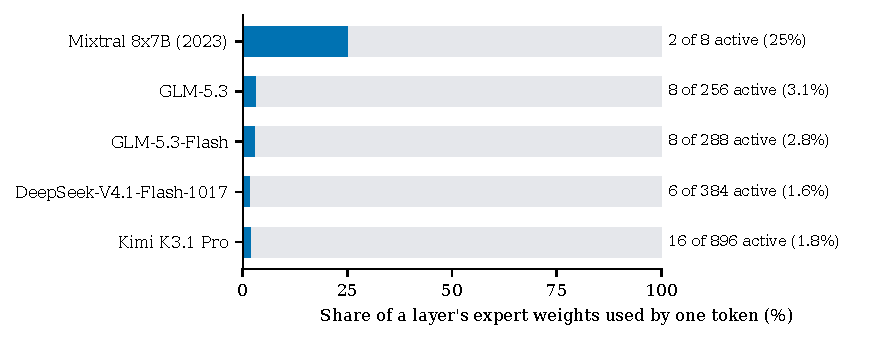
\includegraphics[width=0.8\linewidth]{fig-sparsity.pdf}
  \caption{How little of a layer one token uses. Routed experts per layer and experts active per
  token in four current models: GLM-5.3
  \citep{zai2026glm53}, GLM-5.3-Flash \citep{zai2026glm53flash}, DeepSeek-V4.1-Flash-1017
  \citep{deepseek2026v41flash} and Kimi K3.1 Pro \citep{moonshot2026kimik31}. Values are from each
  model's published configuration.}
  \label{fig:archs}
\end{figure}

\paragraph{The memory problem.} Experts dominate the parameter count, so they decide whether a
model fits. On a machine with unified or GPU memory $M$ smaller than the experts, something
must give, and each family of techniques gives up something different. Pruning gives up
experts. Quantization gives up precision. Offloading gives up time. The hybrids give up a
little of two of these. To compare them we need a description in which all three losses appear
as choices about the same resource.

\section{A common formulation: reach, residency, precision}
\label{sec:space}

\subsection{Three quantities and a rule}

Fix a layer. At token $t$ a deployment is described by:
\begin{itemize}
  \item its \emph{reach} $\reach\subseteq\pool$, the experts the router may select. Pruning
  shrinks reach. Every other technique leaves $\reach=\pool$.
  \item its \emph{resident set} $\res_t\subseteq\reach$, the experts in memory, with
  $|\res_t|=K$. Offloading makes $\res_t$ smaller than $\reach$ and lets it change with $t$.
  \item its \emph{precision} $b_t(e)$ for each resident, the bits per weight it is held at.
  Quantization lowers $b$; mixed-precision schemes make it depend on $e$ and sometimes on $t$.
\end{itemize}
The router's choices under full reach are the \emph{demand},
$D_t=\topk(s,\reach)$. When $D_t\not\subseteq\res_t$ some demanded expert is absent, which we
call a \emph{miss}, and the deployment needs a \emph{miss rule}. Four are in use (Figure~\ref{fig:missrules}), and the offloading literature has compared them as policies for a cache miss \citep{hoang2026specmd,son2026misses}:
\begin{description}
  \item[Wait.] Block the token until the expert has been read. Exact, with latency that depends
  on storage and on the miss rate.
  \item[Substitute.] Keep a second, coarser copy of every expert in memory and serve the miss
  from it. No latency, at the cost of memory for the copies and of the copies' error.
  \item[Re-route.] Serve the token from the best experts that are resident,
  $S_t=\topk(s,\res_t)$, with gates renormalized. No latency and no extra memory, at the cost
  of running an expert the router ranked lower.
  \item[Skip.] Drop the missed choice and renormalize or not. No latency and no memory; the missed choice's contribution is lost.
\end{description}

\begin{figure}[ht]
  \centering
  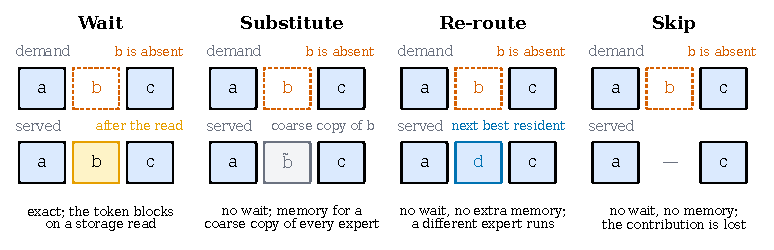
\includegraphics[width=\linewidth]{fig-missrules.pdf}
  \caption{The four miss rules. The router demands experts $a$, $b$ and $c$, and $b$ is not in
  memory. Each rule serves the token differently and pays in a different resource.}
  \label{fig:missrules}
\end{figure}

\subsection{Existing techniques as points}


Table~\ref{tab:corners} places the main techniques. Two observations follow from writing them
this way. First, static pruning is a frozen cache: it is the deployment in which the resident set is
fixed, reach has been cut down to it, and so the question of a miss never arises. Seen from the
full model's router, a pruned model re-routes every token whose demand fell outside the kept
set, and never admits. A fixed resident set is a known baseline among cache policies
\citep{zhang2026reproducible,bacon2026fewer}, and LightMoE notes that a static resident set incurs
misses when the task shifts \citep{luo2026lightmoe}; the formulation states the equivalence outright, so that a pruned checkpoint and an expert cache can be compared directly. Second, the columns are independent. Nothing ties low precision to full
residency, or a dynamic resident set to full precision; those pairings are habits of the
separate literatures. A technique can be low-precision \emph{and} offloaded \emph{and} re-routed,
and the space contains points that none of the families occupies.

\begin{table}[ht]
\centering
\small
\begin{tabular}{@{}lllll@{}}
\toprule
Technique & Reach & Residency & Precision & Miss rule \\
\midrule
Full model & all & all & full & none needed \\
Static pruning \citep{lasby2025reap} & subset & $=$ reach & full & none needed \\
Uniform quantization \citep{tseng2024quipsharp} & all & all & low & none needed \\
Pruning with quantization \citep{chen2025collaborative} & subset & $=$ reach & per expert & none needed \\
Exact offloading \citep{xue2024moeinfinity} & all & subset, dynamic & full & wait \\
Low-precision fetch \citep{tang2024hobbit} & all & subset, dynamic & two levels & wait, shortened \\
Low-precision fallback \citep{chu2025dynaexq} & all & subset $+$ coarse copies & two levels & substitute \\
Cache-aware routing \citep{skliar2024cache} & all & subset, dynamic & full & re-route (biased) \\
Dynamic expert sets \citep{kong2023swapmoe} & all & subset, dynamic & full & re-route \\
Selective fetch \citep{son2026misses} & all & subset, dynamic & low & wait or re-route \\
Nested precision \citep{wei2026matmoe,choi2025slicemoe} & all & all or subset & per expert & substitute \\
\midrule
Routed residency (Section~\ref{sec:method}) & all & subset, dynamic & low, nested & re-route \\
\bottomrule
\end{tabular}
\caption{Memory-constrained MoE techniques described by reach, residency, precision and miss
rule. Entries summarize each method's main configuration.}
\label{tab:corners}
\end{table}

\begin{figure}[ht]
  \centering
  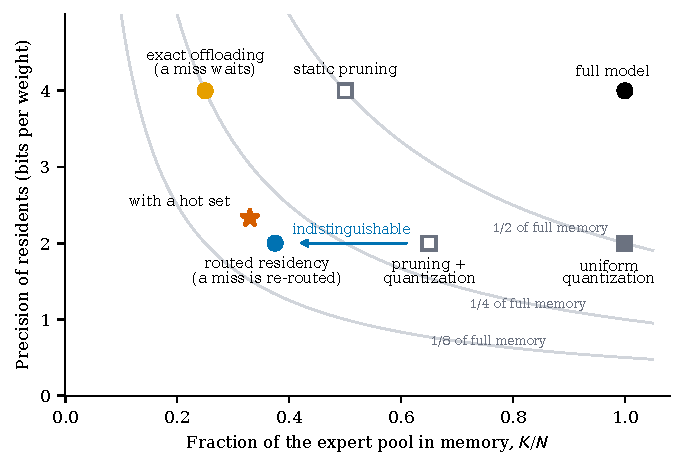
\includegraphics[width=0.8\linewidth]{fig-space.pdf}
  \caption{The design space. Each point is a deployment: the fraction of the expert pool in
  memory and the precision it is held at. Curves are lines of equal memory. Filled markers
  reach the whole pool; hollow markers can use only what they hold. Moving along a curve trades
  residents for bits; the marker's fill is the third axis, and it costs no memory. The arrow
  anticipates a result of Section~\ref{sec:case}: on the tuning texts, a routed set is not separable from a static set about twice its size.}
  \label{fig:space}
\end{figure}

\subsection{One memory account, three costs}

With $L$ layers and $m(b)$ the size of an expert at $b$ bits per weight, the memory a deployment
spends on experts is
\begin{equation}
  M = L\sum_{e\in\res_t} m\bigl(b_t(e)\bigr) \;+\; \text{(any coarse copies)}.
  \label{eq:memory}
\end{equation}
Reach does not appear in Equation~\ref{eq:memory}. An expert that is reachable but not
resident costs storage, not memory, which is what Figure~\ref{fig:space} shows as filled and
hollow markers on the same curve. Besides memory a deployment has three running costs.
\emph{Storage traffic} is the bytes read per token to change the resident set.
\emph{Latency} is the time a token waits; it is zero for every miss rule except waiting.
\emph{Error} is the distance of the output from the full model's. Writing the served
computation as $\hat y=h(x)+\sum_{e\in S_t}\hat g_e\hat f_e(x)$, with $\hat f_e$ the expert at
its held precision, and subtracting Equation~\ref{eq:moe},
\begin{equation}
  \hat y-y \;=\;
  \underbrace{\sum_{e\in S_t}\hat g_e\bigl(\hat f_e(x)-f_e(x)\bigr)}_{\text{coding error}}
  \;+\;
  \underbrace{\sum_{e\in S_t}\hat g_e f_e(x)-\sum_{e\in D_t} g_e f_e(x)}_{\text{routing error}} .
  \label{eq:error}
\end{equation}
The routing error vanishes when the demand is resident, and the coding error vanishes at full
precision. Pruning has only routing error, on every token whose demand left the kept set.
Quantization has only coding error. A deployment that is both low-precision and partly resident
has both, and the question of how to divide memory is the question of which term to shrink.

\FloatBarrier
\section{Routed residency}
\label{sec:method}

Routed residency keeps every expert reachable, holds a changing subset of them in memory at low precision, refines the most used, and re-routes on a miss. Its premise is that the router already computes everything a cache controller needs: its scores say which experts a token wants and how strongly.

\subsection{The policy}

\paragraph{Serving.} The router scores the whole pool. The token is served by
$S_t=\topk(s,\res_t)$ with gates renormalized over $S_t$. If the demand is resident,
$S_t=D_t$ and the layer computes exactly what a uniformly quantized model would.

\paragraph{Admission.} The same scores give the demand $D_t=\topk(s,\pool)$ with gates $g^D$.
Every miss that was demanded strongly,
\begin{equation}
  A_t=\{e\in D_t\setminus\res_t : g^D_e\ge\tau\},
\end{equation}
is read from storage and replaces the resident that has gone longest without a demand of at
least $\tau$. It serves later
tokens. The threshold $\tau$ trades storage traffic against how closely the resident set tracks
demand; $\tau=\infty$ never admits, which is static pruning.

\paragraph{Initial set.} $\res_0$ is the $K$ experts with the most \emph{routed mass}, the sum over calibration text of an expert's gate weight times the norm of its output. This is also how we choose a static set, so that
routed residency and pruning start from the same experts and differ only in admission.

\paragraph{Precision.} Every expert has a code at a base precision. A \emph{hot set} $\hot$ of
$H$ experts per layer, the highest in routed mass, also has a residual code of the base code's
error, and runs at base plus residual when resident. The residual refines the code that is
already in memory. It is not a second copy, so an expert that is promoted or demoted moves only
the residual's bytes, and an expert whose residual is absent still runs.

\paragraph{Skipping.} A served choice with gate below $\delta$ may be skipped. This lowers the
weights evaluated per token and saves no memory.

\begin{algorithm}[t]
\caption{One decode step of a layer under routed residency with settings $(K,\tau,H,\delta)$.}
\label{alg:policy}
\begin{algorithmic}[1]
\State $s\gets\mathrm{router}(x)$
\State $D\gets\topk(s,\pool)$ \Comment{demand: what the full model would run}
\State $S\gets\topk(s,\res)$ \Comment{served set: the best residents}
\State $y\gets h(x)+\sum_{e\in S,\ \hat g_e\ge\delta} \hat g_e\,\hat f_e(x)$ \Comment{$\hat g$: gates renormalized over $S$}
\ForAll{$e\in D\setminus\res$ with $g^D_e\ge\tau$}
  \State in the background, read $e$ from storage into a spare row
  \State point the router at $e$; evict the least recently demanded resident
\EndFor
\State \Return $y$ \Comment{the token never waits for the loop above}
\end{algorithmic}
\end{algorithm}

Algorithm~\ref{alg:policy} states one step. The policy has four settings, and its memory is
Equation~\ref{eq:memory} with $K$ residents at the base size and $H$ residuals. It is also
short in code: Listing~\ref{lst:policy} is the admission loop of the simulator used in
Section~\ref{sec:case}, for one layer of one text (from \src{scripts/runpod/v41_reap/local_eval.py}).

\begin{lstlisting}[float=t, language=Python, caption={The admission loop of our simulator for one layer of one text (abridged, comments added). \texttt{ind} and \texttt{wts} hold each token's demanded experts and gate weights; \texttt{resident} is what the forward pass then serves from.}, label={lst:policy}]
lru = OrderedDict((int(e), None) for e in warm)   # the initial resident set
for t in range(start, start + n):                 # tokens of one text
    row = ind[t].tolist()                         # the experts this token demands
    resident[t, list(lru)] = True                 # what this token may be served from
    for s, e in enumerate(row):
        if wts[t, s] >= thr[e]:                   # demanded strongly
            if e in lru:
                lru.move_to_end(e)                # refresh
            else:
                counts[e, 4] += 1                 # one read from storage
                lru[e] = None                     # admitted: serves from the next token on
                if len(lru) > k:
                    lru.popitem(last=False)       # evict the least recently demanded
\end{lstlisting}

\subsection{Why re-routing is a reasonable miss rule}
\label{sec:why}

Re-routing replaces a demanded expert with one the router ranked lower. Equation~\ref{eq:error} says what that costs within a layer: the routing error grows with the gate weight that was moved and with the difference between the experts involved. Two properties would keep it small. Both can be measured for a model on calibration text, and both hold in the model we study; we do not know how widely they hold.

The first is \emph{concentration}: demand that is far from uniform over the pool. If a small set of
experts carries most of the routed mass, a resident set of modest size serves most choices and
the moved gate weight is small.

The second is \emph{session locality}: the experts a particular text needs form a stable subset of the pool that differs from text to text. A static set must cover the union of all texts'
needs; a dynamic set needs to cover one text's at a time. This is where routed residency can gain over pruning, and it also explains why admission can be lazy: an expert that
arrives a few tokens late is still needed.

\begin{figure}[ht]
  \centering
  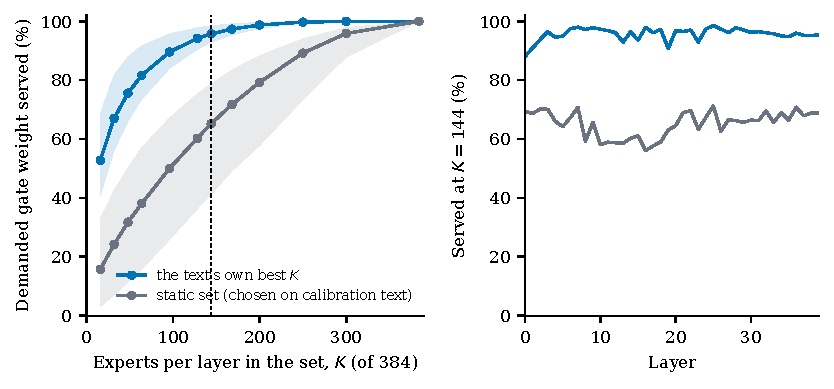
\includegraphics[width=\linewidth]{fig-locality.pdf}
  \caption{Concentration and session locality in the model of Section~\ref{sec:case}. Left: the
  share of a text's demanded gate weight that $K$ experts per layer would serve, for the static
  set chosen on calibration text and for the text's own best $K$; lines are means over 17 texts
  and 40 layers, bands the range over texts. Right: the same at $K=144$, by layer.}
  \label{fig:locality}
\end{figure}

Figure~\ref{fig:locality} measures concentration, and the gap that locality implies, in the model of Section~\ref{sec:case}. The
144 experts per layer that calibration text ranks highest would serve 65\% of a text's
demanded gate weight on average, and between 41 and 79\% depending on the text. The text's own
best 144 would serve 96\% (93 to 98\%; unweighted means over the 17 texts). The text's own set is chosen in hindsight, so the gap between the two curves is what the calibration
set gives up against the best fixed set for that text; a set that changes within the text could serve more still. The gap is present in every layer. Locality does not
mean a small footprint: a text touches about 264 of the 384 experts of a layer at least once,
so the tail of demand is long and thin, which is the case for admitting only on strong demand.

Re-routing also has a failure mode of its own. Substituting a coarse copy keeps the function the router chose and adds noise to it. Re-routing changes \emph{which function} is applied, and when the missed expert was the only one that knew something, the substitute may be confidently wrong. Section~\ref{sec:generation} reports failures consistent with this.

\FloatBarrier
\subsection{The router as the switch}
\label{sec:switch}

\begin{figure}[ht]
  \centering
  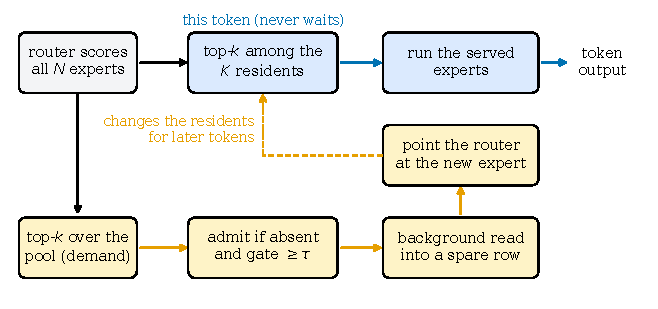
\includegraphics[width=0.82\linewidth]{fig-system.pdf}
  \caption{One layer under routed residency. The blue path produces the token and depends only
  on what is already in memory. The orange path changes what will be in memory for later
  tokens.}
  \label{fig:system}
\end{figure}

A policy that never waits is only useful if it can be implemented without stalling a decoder,
and in particular without the decode path taking a lock or stopping to copy a result from the GPU back to the CPU program that drives it (the \emph{host}). The following construction (Figure~\ref{fig:system}) does this. We built it in one runtime; it uses nothing beyond an MoE layer written as a router followed by a gather over a stacked array of experts.

Hold the residents of a layer as rows of one stacked array per projection, with a few spare
rows. Keep the router's weights for the whole pool. Give every absent expert a router bias of
$-\infty$: the top-$k$ over the biased scores is then the served set, and the top-$k$ over the
unbiased scores is the demand, from one router evaluation. Installing or evicting an expert
changes one bias and one entry of an expert-to-row table. The decode graph itself never
changes shape.

Three ordering rules make an install safe. An evicted row's bias is set to $-\infty$ first, so
nothing routes to it. The row is overwritten only after every decode call that was issued
before the eviction has finished. The router is pointed at the new expert only after its bytes
are in place. A token therefore never waits for a read and never runs a partly written expert.
The demand is an output of the token's own computation and can be read lazily, after the
fact, so observing it does not make the decoder stop and wait either.

\begin{figure}[ht]
  \centering
  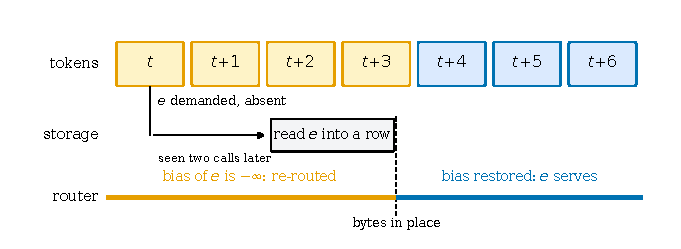
\includegraphics[width=0.86\linewidth]{fig-timeline.pdf}
  \caption{The life of one admission. Expert $e$ is demanded at token $t$ and is absent. The
  policy sees the demand two decode calls later and reads $e$ into a row that no earlier call
  can still route to. Tokens are served by re-routing meanwhile; once the bytes are in place,
  the router's bias for $e$ is restored and $e$ serves.}
  \label{fig:timeline}
\end{figure}

Listing~\ref{lst:switch} shows these rules in our implementation
(\texttt{install} and \texttt{evict} from \src{scripts/v41_build/omlx_routed.py},
\texttt{route} and \texttt{unroute} from \src{scripts/v41_build/omlx_lattice.py}), and
Figure~\ref{fig:timeline} lays the same sequence out in time. The switch itself is two
assignments. An eviction only clears the bias and puts the row on a cooling list; the row is
reused for a read once the call being built at that moment is known to have finished, and
\texttt{install} restores the bias only when every read of the expert has completed.
Appendix~\ref{app:code} gives the kernel that takes both selections from one set of scores.

\begin{lstlisting}[float=t, language=Python, caption={The router switch and the install and evict steps of our implementation (abridged: statistics and the error check on each read removed). \texttt{OFF} is a bias of $-10^{30}$.}, label={lst:switch}]
def route(self, layer, expert, slot):
    layer.slot_map[expert] = slot
    if layer.hot:  # in place, so Experts._hot sees it too
        layer.hot_of_slot[slot] = layer.hot.get(expert, NO_RESIDUAL)
    layer.gate.bias[expert] = float(layer.pool_bias[expert])

def unroute(self, layer, expert, slot):
    layer.gate.bias[expert] = OFF

def install(self, layer) -> None:
    """Route the experts whose bytes have landed. The router arrays are replaced, never
    written in place and never evaluated here: calls already built keep the old ones, and
    the next call's own eval computes the new ones without a wait."""
    done = [e for e, (_, futures) in layer.reading.items() if all(f.done() for f in futures)]
    for expert in done:
        slot, futures = layer.reading.pop(expert)
        self.route(layer, expert, slot)
        layer.slot_expert[slot], layer.slot_of[expert] = expert, slot
        layer.last_use[slot] = self.step

def evict(self, layer, protected) -> None:
    """Unroute the least recently demanded residents until ``spare`` slots are free or coming."""
    short = self.spare - len(layer.free) - len(layer.cooling)
    if short <= 0:
        return
    order = np.argsort(layer.last_use, kind="stable")
    victims = [int(s) for s in order if layer.slot_expert[s] >= 0 and int(layer.slot_expert[s]) not in protected]
    for slot in victims[:short]:
        expert = int(layer.slot_expert[slot])
        del layer.slot_of[expert]
        layer.slot_expert[slot] = -1
        layer.last_use[slot] = np.inf
        self.unroute(layer, expert, slot)
        # Calls built before this one may still route here; its bytes may change only once
        # the call being built now is known to have finished.
        layer.cooling.append((slot, self.step))
\end{lstlisting}

Two properties follow from this construction and bound what the policy can do. An admitted
expert serves a few tokens after it was demanded, not the next token. And the resident set is
fixed within a single forward pass, so it cannot adapt inside the processing of a prompt or
inside a multi-token verification step of speculative decoding. Both argue for a good initial
set, a point Section~\ref{sec:admission} returns to.

\FloatBarrier
\section{Allocating memory: an order of spending}
\label{sec:principle}

Equation~\ref{eq:error} splits the error into a routing term and a coding term, and
Equation~\ref{eq:memory} prices both in the same unit. Suppose experts are ranked by routed
mass, with $\rho_i$ the share of the $i$-th. A gigabyte can be spent in two ways.

\emph{As residents.} It holds $1/(L\,m_b)$ more experts per layer at the base precision. The
choices it converts from re-routed to served are those of the experts just outside the resident
set, and the gain is roughly their share of demand times the penalty $\sigma$ of serving a
choice from a substitute:
\begin{equation}
  \text{gain per byte as residents} \;\approx\; \frac{\rho_{K}\,\sigma}{L\,m_b}.
\end{equation}

\emph{As bits.} It gives $1/(L\,m_r)$ more experts a residual. The gain is their share of demand
times the drop in coding error $\varepsilon(b)-\varepsilon(b')$ from the refinement:
\begin{equation}
  \text{gain per byte as bits} \;\approx\; \frac{\rho_{H}\,\bigl(\varepsilon(b)-\varepsilon(b')\bigr)}{L\,m_r}.
\end{equation}
This is a heuristic and not a theorem; it ignores interactions between layers and between the
two terms. It is nevertheless enough to predict an order, because the gain from residents falls as the resident set grows while the gain from the first residuals does not.

\begin{enumerate}
  \item \textbf{Precision first, up to the knee of the code.} Coding error need not fall smoothly with bits. If below some precision a code stops preserving what an expert computes, $\varepsilon$ there is so large that holding the expert is worth little, and until every held expert is past that knee, bits beat anything else. Two studies of other models and codes locate such a knee: \citet{jha2026half} finds that a half-pruned model beats the full model quantized to the same size only where the full model would need fewer than 3 bits per weight, and ProQuant \citep{chen2026proquant} replaces the 1-bit option of a mixed-precision search with removal of the expert.
  \item \textbf{Then reach, for free.} Reach is absent from Equation~\ref{eq:memory}. Letting
  the router select from the whole pool costs storage and admission traffic, not memory, and it
  turns the fixed routing error of a pruned model into one that shrinks as the resident set follows the text.
  \item \textbf{Then residents.} While the resident set is small, the experts just outside it
  still carry a real share of demand, $\rho_K$ is large, and each one admitted removes
  routing error on many choices. Residents win for as long as a substitute's penalty
  $\sigma$ outweighs a bit's worth of coding error on the experts already held.
  \item \textbf{Then bits again.} Under concentration $\rho_K$ falls with $K$, while $\rho_H$ for the first few experts stays large. Past some $K$ the next resident serves little demand, and a residual on the most used experts is the better purchase. The hot set this
  implies is small, since the gain per residual falls with $\rho_H$ as well.
\end{enumerate}

\begin{figure}[ht]
  \centering
  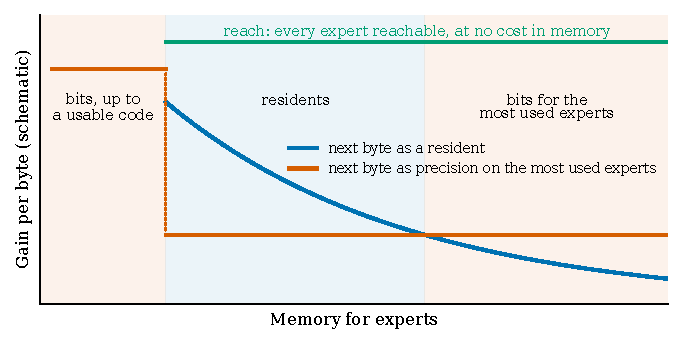
\includegraphics[width=0.8\linewidth]{fig-order.pdf}
  \caption{The order of spending, as a schematic of the two gains. Below the knee of the code,
  precision comes first. Past it, the gain from the next resident starts high and falls as the
  resident set grows, while the gain from precision on the most used experts stays roughly
  level; where they cross, spending switches. Reach costs no memory at any budget. The curves
  are illustrative, not measured.}
  \label{fig:order}
\end{figure}

Figure~\ref{fig:order} draws this order. The middle of it runs against the habit of keeping
fewer experts at higher precision:
between the knee of the code and the point where most demand is served from memory, the error model above predicts that more experts beat better experts. SliceMoE makes the same observation for an expert
cache \citep{choi2025slicemoe}, and general results on compression favor more parameters at lower
precision down to about 4 bits \citep{dettmers2022case,kuzmin2023pruning}. Our error model adds where the preference begins, at the knee, and where it ends.

\paragraph{When the order should hold.} The argument needs four conditions. (i) The pool is
wide and activation sparse, $k\ll N$, so that a resident set much smaller than the pool still
offers good substitutes. (ii) Demand is concentrated and local to a session, so that
$\rho_K$ falls quickly and the resident set can follow it. (iii) A base code exists past the
knee at a size that leaves room for breadth. (iv) Storage is fast enough to carry the admission
traffic at the decoding speed. The current models in Figure~\ref{fig:archs} all have the wide, sparse pools that (i) starts from, with 256 to 896 experts per layer and 1.6 to 3.1\% of them active. We expect the order to fail for narrow pools: with eight experts and two active, removing
residents removes a quarter of the layer at a time, substitutes are poor, and precision should
come first throughout.

\paragraph{What the order predicts.} For a model that meets the conditions: a routed set
should beat a static set of the same size at every budget, by more at small budgets; a coarser
code than the knee should lose to fewer experts at a finer one; a hot set should not be worth its memory at small budgets and should be at large ones; and the hot set should be small. The case study
tests each of these.

\FloatBarrier
\section{Case study: a 384-expert model on a 128\,GB laptop}
\label{sec:case}

\subsection{Setup}
\label{sec:setup}

\paragraph{Model and codes.} DeepSeek-V4.1-Flash-1017 \citep{deepseek2026v41flash} has 40 MoE
layers, each with 384 routed experts of which six are active. Its routed experts hold 544
billion parameters, 289\,GB at the released precision of 4.25 bits per weight (written 4 bits
below), so they do not fit in 128\,GB at that precision, nor at 2 bits (141\,GB). The released
model is our reference, the \emph{full model}; an expert at 4 bits has no error by
construction. Every expert is coded once at 2 bits with the E8P lattice codebook of QuIP\#
\citep{tseng2024quipsharp}, and the hot set's residuals are 1-bit lattice codes of the 2-bit
code's error. We count 9.2\,MB for a 2-bit expert, 4.6\,MB for a residual and 18.8\,MB for a 4-bit expert. Hot sets are drawn from the 192 experts for which 4-bit weights and residuals were available (Appendix~\ref{app:setup}).

\paragraph{Baselines.} A \emph{static set} is the $K$ experts with the most routed mass at 2
bits, never changed: pruning with our codes, and routed residency with $\tau=\infty$. The
\emph{pruned checkpoint} is the model pruned with REAP \citep{lasby2025reap} to 192 experts per
layer and kept at 4 bits; its 192 experts recoded at 2 bits are the \emph{pool of 192}.

\paragraph{Measurement.} Quality is the KL divergence from the full model's next-token
distribution to the compressed model's, in nats, with both models given the same preceding text at every position (teacher forcing), on the first 1{,}024 tokens of
evaluation text from ten domains (code, shell, security, networking, business, chat and
prose), 17 distinct texts in all; calibration text is separate. The quantity is $\sum_{x\in A} p(x)\log\bigl(p(x)/q(x)\bigr)$, with $p$ and $q$ the full-vocabulary probabilities of the full and the compressed model and $A$ the 2{,}048 tokens the full model rates most probable at that position. It is a partial sum of the KL divergence, not the divergence between the two distributions renormalized on $A$: it does not see probability that the compressed model puts outside $A$, and at a single position it can be negative, as it is at 18\% of positions for routed residency with 144 residents, never below $-0.06$. We call it KL throughout; where a comparison turns on hundredths of a nat, this is one more reason for caution. Differences are paired by text
with a 95\% bootstrap interval over texts in brackets. One text carries a fifth of the weight, because four sessions share it, so the effective sample is about 12 texts. We report several dozen paired comparisons and correct none for multiplicity; an interval that barely excludes zero should be read with that in mind. Policies are compared in a simulator
that runs the real forward pass with the residency decisions of Algorithm~\ref{alg:policy}
applied per token and layer. The simulator installs an admitted expert one token after it is demanded and adapts within a text; the served system of Section~\ref{sec:serving} installs later and holds its set fixed while it reads a prompt; Section~\ref{sec:serving} gives the simulator that timing and reports what it costs. Appendix~\ref{app:setup} gives the details, including an
eleventh domain that we exclude and why.

\subsection{Reach: routed residency against static sets}
\label{sec:frontier}

\begin{figure}[ht]
  \centering
  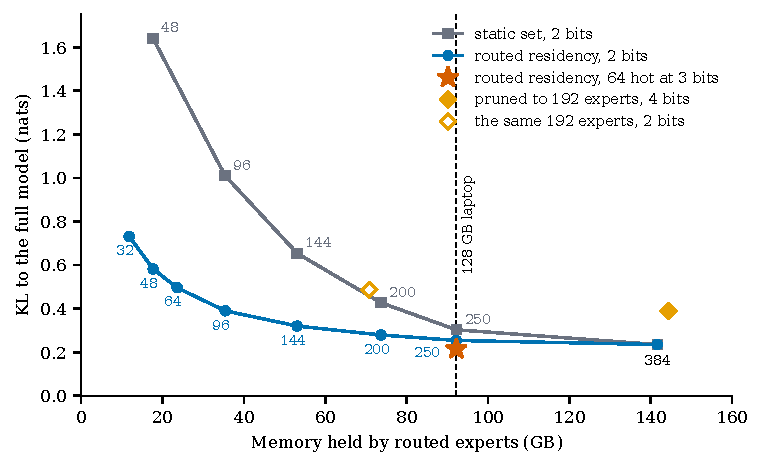
\includegraphics[width=0.84\linewidth]{fig-frontier.pdf}
  \caption{Case study: distance to the full model against the memory held by routed experts.
  Both curves use the same 2-bit codes and the same number of experts in memory, marked on each
  point; the routed set may exchange its experts for others in the pool, the static set may
  not. Diamonds are the pruned checkpoint at 4 bits and its experts at 2 bits. The star is
  routed residency with a third bit on 64 hot experts. The dashed line is the expert memory of a 128\,GB machine; points there are simulated, and the largest configuration we served held 200 residents.}
  \label{fig:frontier}
\end{figure}

\begin{table}[ht]
\centering
\small
\begin{tabular}{@{}rrccl@{}}
\toprule
Residents $K$ & Memory & Static set & Routed residency & Difference \\
\midrule
 48 &  18\,GB & 1.640 & 0.582 & $-1.058$ \ci{-1.365}{-0.832} \\
 96 &  35\,GB & 1.010 & 0.390 & $-0.619$ \ci{-0.829}{-0.460} \\
144 &  53\,GB & 0.654 & 0.320 & $-0.333$ \ci{-0.472}{-0.229} \\
200 &  74\,GB & 0.427 & 0.279 & $-0.148$ \ci{-0.246}{-0.078} \\
250 &  92\,GB & 0.303 & 0.254 & $-0.048$ \ci{-0.092}{-0.016} \\
384 & 141\,GB & 0.235 & 0.235 & \\
\bottomrule
\end{tabular}
\caption{Case study: KL to the full model (nats) for a static set and for routed residency
with the same number of experts per layer in memory, at 2 bits.}
\label{tab:frontier}
\end{table}

The first prediction holds (Figure~\ref{fig:frontier}, Table~\ref{tab:frontier}). With
identical codes and the same number of experts in memory, routed residency is closer to the
full model than a static set at every budget, and the gap grows as memory shrinks. Read along
the memory axis, on these texts a routed set is not separable from a static set 1.7 to 2.1 times its size: 96 routed residents against
200 static ones ($-0.037$ \ci{-0.136}{+0.034}), and 144 against 250
($+0.017$ \ci{-0.026}{+0.051}). These are failures to separate at 17 texts, not tests of equivalence, and the held-out texts below qualify them.

Two comparisons isolate the value of reach from that of residency. Holding residency at 144 and widening the
pool, from the pool of 192 to all 384 experts, lowers KL from 0.499 to 0.307 at an admission threshold of 0.2 ($-0.192$ \ci{-0.272}{-0.128}), although the added experts occupy no memory until they are asked for. The two runs differ in more than reach: each starts from the 144 experts that its own calibration statistics rank first, and the two starting sets share 108 of 144 experts per layer, so part of the difference may belong to the starting set. And 144 residents drawn from the whole pool at the default threshold, in 53\,GB, are closer to the full model than the entire pool of 192 held in memory at once in 71\,GB (0.320 against 0.486, $-0.166$ \ci{-0.232}{-0.115}). Reaching a wide pool is worth more than holding a
narrow one.

\paragraph{Held-out texts.} The settings above were chosen on the 17 texts they are reported
on. We therefore froze them and scored 36 further texts, each up to its first
8{,}192 tokens (Table~\ref{tab:heldout}). No threshold, hot set or budget was chosen on these texts, but they are not untouched: they belong to the 54 sessions on which the rule that ranks experts by routed mass was compared with the pruning method's own (Appendix~\ref{app:setup}). Routed residency beats the static set of the same
size by more than on the tuning texts: $-0.503$ \ci{-0.631}{-0.383} at 144 residents, in 35 of
36 texts, and $-0.793$ \ci{-0.969}{-0.629} at 96, in all 36. Two of the five budgets were rescored; at both, the comparison at equal size
does not depend on the texts the settings were chosen on. Nor does it depend on text the policy could have met before. Five of the 36 texts open with a run of 64 or more tokens that also opens a calibration or tuning text: shared code context at the head of two long sessions, shorter openings of two more, and one chat prompt repeated whole. Those runs hold 8{,}982 of the 49{,}990 scored positions. Without them, and without the text they leave empty, the differences are $-0.521$ \ci{-0.648}{-0.400} at 144 residents and $-0.795$ \ci{-0.970}{-0.627} at 96.

In absolute terms the held-out texts are harder. The whole pool scores 0.373 (0.235 on the tuning texts), routed residency with 144 residents 0.715 (0.320), and static sets of 144 and 250 score 1.218 and 0.598 (0.654 and 0.303). The comparison with larger static sets does not survive intact. 96 routed residents are not separable
from 200 static ones ($+0.069$ \ci{-0.044}{+0.190}), but 144 are worse than
250 ($+0.117$ \ci{+0.025}{+0.220}, better in 9 of 36 texts) and not separable from 200 ($-0.090$ \ci{-0.198}{+0.019}). The held-out texts are short, with a median of 213.5 scored
positions, where the tuning texts all have 1{,}023. Splitting them by length, a split we chose after seeing these results, suggests why: the routed set starts as the static set and needs demand to
depart from it. On texts under 256 positions it is 0.54 from holding the whole pool and worse than 250 static residents; from
1{,}024 positions on it is 0.075 from the whole pool, close to the 0.086 of the tuning texts, and
not separable from 250 static residents, though better in only 1 of those 7 texts. Reach is worth less than a factor of two in memory on short texts and may approach it on long ones; these data do not establish the second. A short text ends before admission has replaced much of the starting set, so it is served largely by experts chosen for other text; Section~\ref{sec:admission} returns to this gap.

The same positions were also scored, in the comparison of ranking rules of Appendix~\ref{app:setup}, for two static sets of 192 at 4 bits, each 144\,GB of experts: the 192 experts of largest routed mass score 0.741 and the pruned checkpoint 0.814. Routed residency with 96 residents at 2 bits, in 35\,GB, is worse than the first ($+0.134$ \ci{+0.013}{+0.253}) and not separable from the second ($+0.060$ \ci{-0.047}{+0.175}); with 144 residents, in 53\,GB, it is not separable from the first ($-0.025$ \ci{-0.141}{+0.087}) and better than the second ($-0.099$ \ci{-0.191}{-0.008}). These rows come from another evaluation harness, at the released 4-bit precision, and cost three to four times the expert memory; they are the strongest static baselines we have on these texts, and at the smaller budget the routed set does not match the better of them.

\begin{table}[ht]
\centering
\small
\begin{tabular}{@{}lrlll@{}}
\toprule
Scored positions & Texts & Against static 144 & Against static 250 & Against the whole pool \\
\midrule
under 256      & 19 & $-0.486$ \ci{-0.603}{-0.369} & $+0.238$ \ci{+0.092}{+0.408} & $+0.543$ \ci{+0.372}{+0.741} \\
256 to 1{,}023 & 10 & $-0.709$ \ci{-1.043}{-0.391} & $-0.055$ \ci{-0.162}{+0.030} & $+0.148$ \ci{+0.102}{+0.200} \\
1{,}024 and over & 7 & $-0.255$ \ci{-0.402}{-0.123} & $+0.032$ \ci{-0.011}{+0.072} & $+0.075$ \ci{+0.045}{+0.110} \\
\midrule
all            & 36 & $-0.503$ \ci{-0.631}{-0.383} & $+0.117$ \ci{+0.025}{+0.220} & $+0.342$ \ci{+0.234}{+0.470} \\
\bottomrule
\end{tabular}
\caption{Held-out texts: KL of routed residency with 144 residents minus KL of a static set of
144, of a static set of 250, and of the whole pool in memory, by the length of the text.
Settings frozen before scoring; the length split was chosen after the results were seen.}
\label{tab:heldout}
\end{table}

\begin{figure}[ht]
  \centering
  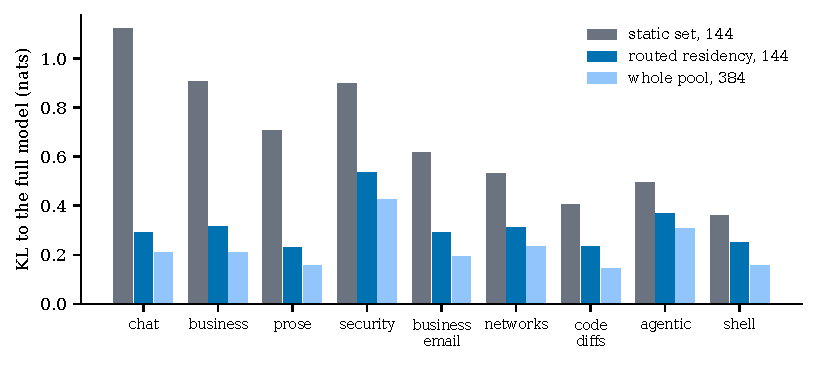
\includegraphics[width=0.92\linewidth]{fig-domains.pdf}
  \caption{Case study: KL to the full model by domain with 144 experts per layer in memory, for
  a static set and for routed residency, and with the whole pool in memory. Domains are ordered
  by the gap between the first two. The two agentic domains share their first 1{,}024 tokens
  and are shown once.}
  \label{fig:domains}
\end{figure}

Figure~\ref{fig:domains} breaks the comparison down by domain. The static set loses most to
routed residency on chat, business text and prose; chat and prose are among the domains with
the least calibration text. Routed residency recovers most of that loss; on agentic coding and shell sessions the two are
closest. In every domain routed residency lies between the static set and the whole pool.

The price is reads from storage: 2.6 experts admitted per token at 144 residents, and more as memory shrinks.

\FloatBarrier
\subsection{Residents against bits}
\label{sec:bits}

\begin{figure}[ht]
  \centering
  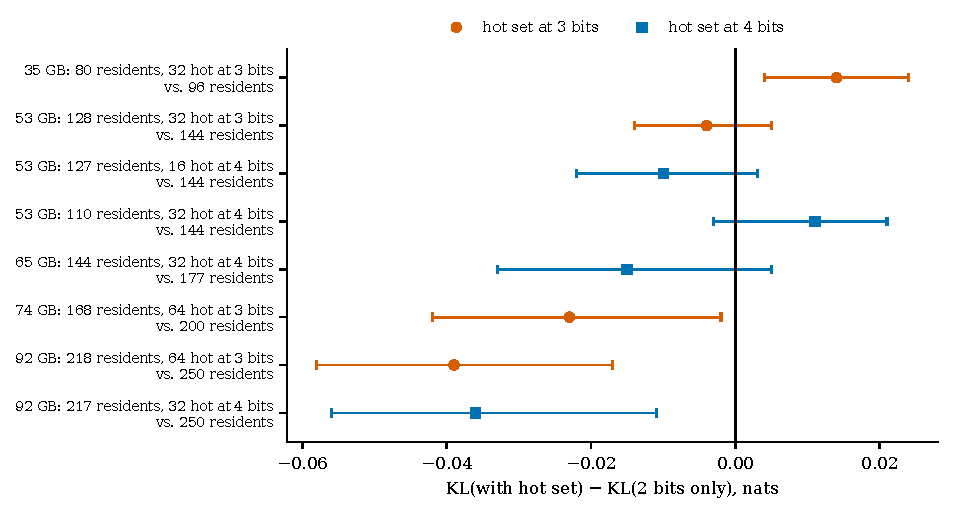
\includegraphics[width=0.9\linewidth]{fig-bits.pdf}
  \caption{Case study: more bits against more residents at equal expert memory. Each row
  removes residents from a 2-bit configuration and spends their memory on a hot set. Points are
  the paired difference in KL, bars the 95\% interval over texts; left of zero, bits win.}
  \label{fig:bits}
\end{figure}

\paragraph{Below the knee.} With our codes the knee lies between 1 and 2 bits. Inside the pool of 192, all
192 experts at 1 bit are far worse than 96 experts at 2 bits in the same memory (1.172 against
0.801). A design built on 1-bit codes, with every expert of that pool resident at 1 bit and a routed set of 1-bit residuals on top, so that a miss runs at 1 bit, does no better than a static set at flat 2 bits in the same memory
($-0.020$ \ci{-0.067}{+0.018}).

\paragraph{Above it.} Figure~\ref{fig:bits} holds memory fixed and moves it from residents to
a hot set, at 3 bits with the nested residual and at the released 4 bits as an upper bound on
what extra bits can buy. The third prediction is not contradicted: above the residency floor a third bit is never worse than more residents, and from 74\,GB it is better. At 35\,GB, giving up 16 of 96 residents for a third bit
on 32 hot experts makes the model worse ($+0.014$ \ci{+0.004}{+0.024}). At 53\,GB the same
trade is level ($-0.004$ \ci{-0.014}{+0.005}), and so are hot sets at 4 bits at 53 and
65\,GB. At 74\,GB a hot set of 64 wins ($-0.023$ \ci{-0.042}{-0.002}), and at 92\,GB it wins
clearly ($-0.039$ \ci{-0.058}{-0.017}). The tested allocations change rank between 53 and 74\,GB. The configurations with a hot set at those budgets hold 128 and 168 residents, 33 and 44\% of the pool, and the 2-bit alternatives 144 and 200, 38 and 52\%; two pairs do not place a crossover more closely than that. Past it, 168 residents with a hot set in 74\,GB are indistinguishable from 250 residents at 2 bits in 92\,GB ($+0.001$ \ci{-0.018}{+0.023}). The residents' side of the order rests on the one budget below the crossover, and that budget is also below the residency floor of Section~\ref{sec:generation}; above the floor we saw ties and then wins for bits. The hot-set sizes were chosen on these texts and were not rescored on held-out text, and the interval of the win at 74\,GB ends at $-0.002$. The hot set need not be large: at 92\,GB, 32, 64 and 96 hot experts per layer are within 0.01 of one another. A third bit
does what the 4-bit weights do at equal memory ($-0.004$ \ci{-0.009}{+0.004}), so the nested
residual loses nothing to a separate high-precision copy. Appendix~\ref{app:bits} gives every
configuration.

\paragraph{The opposite allocation.} The pruned checkpoint spends its memory the other way:
half the pool at 4 bits, in 144\,GB. It scores 0.389 with its 4-bit weights decoded and run through the same computation as our other rows, and 0.393 on its own 4-bit path ($-0.004$ \ci{-0.009}{+0.002} between the two); we use the first, against 0.235 for the whole pool at 2
bits in 141\,GB, and against 0.303 for a static set of 250 at 2 bits in 92\,GB.
The pruned checkpoint also differs from our static sets in which experts it keeps. At 2 bits its 192 experts and the 192 with the most routed mass are not distinguishable on this metric (0.486 against 0.456, $-0.030$ \ci{-0.095}{+0.051}), an interval wide enough that the choice of experts could account for part of the gap; with tool use included the two differ by 0.17 nats (0.747 against 0.579). At the released 4 bits the precision is held equal. Scored against the full model on one GPU, in a harness that reproduces the pruned checkpoint's 0.389 to within 0.003, the 192 experts of largest routed mass score 0.336 and the pruned checkpoint's 192 score 0.392 ($-0.056$ \ci{-0.122}{+0.026}, lower in 13 of 17 texts). The choice of experts is again not separable; the precision is. The same 192 lose 0.120 \ci{0.099}{0.143} going from 4 to 2 bits, in every text. Routed residency with 144 residents at 2 bits, in 53\,GB, is not separable from that static set at 4 bits in 144\,GB ($+0.016$ \ci{-0.059}{+0.118}).

\FloatBarrier
\subsection{Admission and the initial set}
\label{sec:admission}

\begin{figure}[ht]
  \centering
  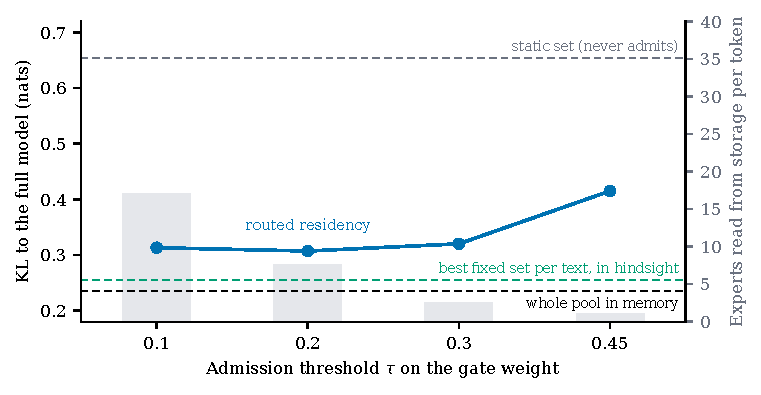
\includegraphics[width=0.8\linewidth]{fig-admission.pdf}
  \caption{Case study: the admission threshold at 144 residents. The line is KL to the full
  model; bars are experts read from storage per token. Dashed lines mark a static set, the best
  fixed set for each text chosen with hindsight, and the whole pool in memory.}
  \label{fig:admission}
\end{figure}

Quality is flat in the admission threshold over a wide range (Figure~\ref{fig:admission}). At
144 residents, thresholds of
0.1, 0.2 and 0.3 on the gate weight give 0.313, 0.307 and 0.320, while storage traffic falls
by a factor of six; 0.45 starves the resident set (0.415).

What remains to be gained is not in the admission rule. A fixed set of 144 experts chosen for each text with hindsight scores 0.255, which is 0.020 \ci{0.012}{0.027} from holding the whole pool and 0.065 \ci{0.050}{0.083} better than admission at $\tau=0.3$. This is evidence of session locality: over the 1{,}024 tokens we score, a fixed 144 of the 384 experts per layer serve a text nearly as well as the whole pool. What routed residency lacks is knowing those experts at the start. The two constraints of Section~\ref{sec:switch} make that costly: an admitted expert serves only a few tokens after it was demanded, and none is admitted while a prompt is read.

We tried to close the gap by learning one threshold per expert from calibration data, twice:
once minimizing the strongly demanded gate weight left unserved, and once using a cost per
missed expert measured through the model. Each fit improved its own objective on held-out text,
and neither improved the model (Appendix~\ref{app:admission}). A cost measured while experts were missed at random does not describe the misses of a policy fitted to exploit that cost. We conclude that
effort is better spent on predicting a text's experts from its prompt than on the admission
rule.

\FloatBarrier
\subsection{A running system}
\label{sec:serving}

We implemented the construction of Section~\ref{sec:switch} inside an existing MLX
\citep{mlx} runtime for this model \citep{omlx}, without modifying the runtime, on an Apple M4
Max with 128\,GB. Figure~\ref{fig:speed} separates what waiting costs from what routed residency costs.

\begin{figure}[ht]
  \centering
  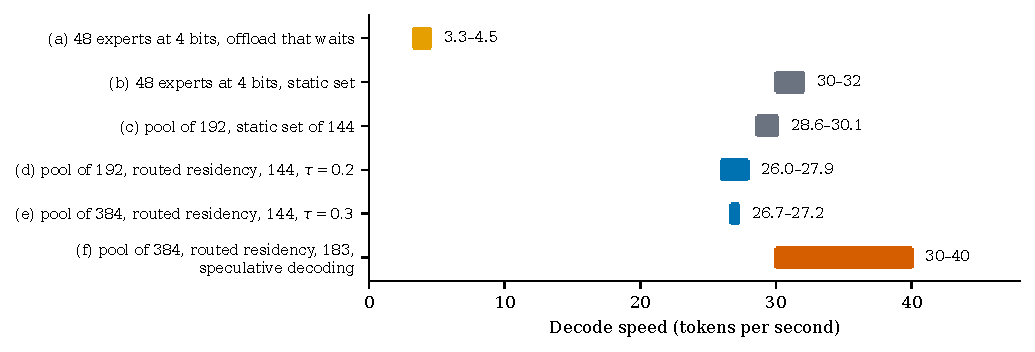
\includegraphics[width=0.9\linewidth]{fig-speed.pdf}
  \caption{Case study: decode speed. Bars (a) to (e) are ranges over greedy requests of 250 to
  1{,}200 tokens on a short prompt (a third request for (e), 310 tokens after a 4{,}341-token
  prompt, ran at 23.0 and is not drawn); (f) is the range of median speeds over four runs of sampled requests. Pools
  of 192 and 384 are at 2 bits.}
  \label{fig:speed}
\end{figure}

Configurations (a) and (b) hold the same number of experts in the same memory: the runtime's waiting offload, which as implemented also leaves its fused decode path, is seven times slower than a static set. Configurations (c) and (d) compare routed residency with a static set drawn from the same pool: 7 to 9\% slower, for scoring the demand and installing about two experts per token. Reaching the whole pool costs no more at $\tau=0.3$ (e); at $\tau=0.2$ it admits about three times as many experts and was up to 15\% slower. These ranges cover two or three requests each, and the median speed of one configuration varied by up to 25\% between runs (Appendix~\ref{app:serving}), more than the difference reported here. A repeat with five server launches of each configuration in turn, 144 residents from the whole pool and no speculative decoder, does not find the cost: the static set decoded at a median of 27.5 tokens per second on each of two short requests and at 26.4 after a 4{,}341-token prompt, routed residency at 28.3, 28.9 and 28.0, and the ranges overlap. Routed residency costs no decode speed that we can resolve. With the model's speculative decoder the whole pool is served at 30
to 40 tokens per second (f). The same runtime serves the pruned checkpoint with its waiting offload at 5.6 to 6.3 tokens per second, but that run differs in checkpoint, precision and decoder, and we do not offer the ratio as a comparison of systems. We have no measurement of another runtime at equal memory on this model; the wait rules of our own code path are measured in Section~\ref{sec:dial}. The hot set is not free in a running system: 64 hot
experts at 3 bits decode 11\% slower at equal memory, so the served configuration is 2-bit
only. Appendix~\ref{app:serving} has the details.

The divergences of this paper come from a simulator that installs an expert one token after its demand and lets the resident set change inside a prompt. The served system reads the demand two decode calls late, then reads from storage, and holds its set while it reads a prompt. We gave the simulator that timing: an admission lands three tokens after its demand, and none lands during the first 256 tokens of a text, a quarter of the scored window. The delay alone costs 0.045 \ci{0.034}{0.056} at 96 residents, 0.023 \ci{0.020}{0.028} at 144 and 0.009 \ci{0.000}{0.022} at 200. With the opening frozen as well, 96 residents score 0.612 and 144 score 0.442, which is 0.222 \ci{0.170}{0.291} and 0.121 \ci{0.088}{0.168} above the simulator's own timing and still 0.397 \ci{0.287}{0.543} and 0.212 \ci{0.138}{0.309} below static sets of those sizes. The comparison with static sets survives the served timing at about two thirds of its size. The larger part of the loss is the frozen opening, which admitting between the chunks of a prompt would address, and not the delay. These are simulator rows under the served timing; we still have no divergence measured on the served system itself.

\FloatBarrier
\subsection{A limit: the residency floor}
\label{sec:generation}

\begin{figure}[ht]
  \centering
  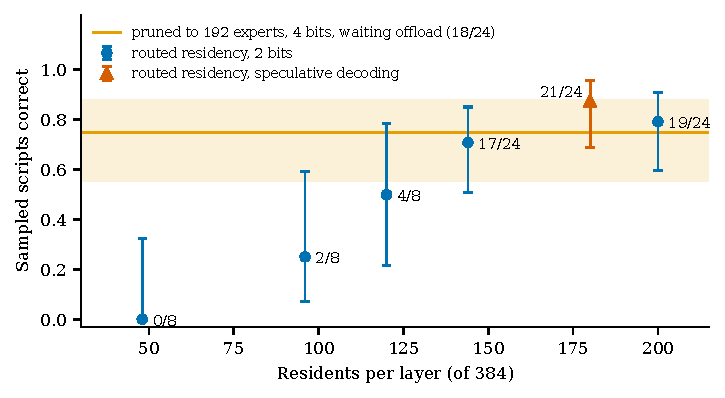
\includegraphics[width=0.8\linewidth]{fig-generation.pdf}
  \caption{Case study: sampled scripts that run correctly against residents per layer. Counts
  are correct samples of 8 or of 24; bars are 95\% Wilson intervals. The line and band are the
  pruned checkpoint at 4 bits (18 of 24). The triangle is routed residency with speculative
  decoding, the square a static set of the same 2-bit experts with that decoder off.}
  \label{fig:generation}
\end{figure}

KL is measured with the full model's context forced at every position. To see whether it predicts what the model does when it continues from its own output, we sampled one coding request at the model's recommended
settings and counted the scripts that run and give the right output
(Figure~\ref{fig:generation}).

With 144 or more residents, routed residency is not separable from the pruned checkpoint at
4 bits (17 to 21 correct of 24, against 18). A static set of 144, the same codes in the same memory with admission switched off, gets 9 of 24 with the speculative decoder off, the condition under which routed residency at that size got 17 ($p=0.04$, Fisher's exact test), and 4 of 24 with it on, where routed residency scored 5 of 8 at that size ($p=0.023$) and 21 of 24 at 180 residents. The gap is specific to this request. On two further script requests, 16 samples a row at 144 residents with the decoder off, routed residency gives 10 and 16 correct and the static set 12 and 12 ($p=0.70$ and $0.10$). One request of three separates the two, and we do not claim that a static set of this size generates worse in general. Below 144 residents KL does not predict the outcome on this prompt. At 96 residents neither KL nor the change in the loss on the text separates routed residency from the pruned checkpoint (0.390 against 0.389, $+0.002$ \ci{-0.075}{+0.058}; 0.081 against 0.095 nats of added loss), yet 4 of 24 samples are correct against 18 of 24 ($p=0.0001$), and at 48 none of 8 is. The failures are mostly misspelled identifiers and answers that never finish, and neither a lower temperature nor a truncated sampling tail raises the counts. They
track the share of demand that is re-routed: 35\% at 48 residents, 25\% at 96, 10\% at 200,
where no failure is a misspelling.

This is consistent with the failure mode anticipated in Section~\ref{sec:why}, although we did not trace individual wrong tokens to re-routed choices. Our hypothesis is that a re-routed choice occasionally yields a confidently wrong token. Such errors would be concentrated in a few positions, so that an average divergence under forced context barely registers them while free-running generation cannot recover from them. The order of Section~\ref{sec:principle} therefore applies above a \emph{residency floor}, here between 96 and 120 of 384 experts per layer: 14 of 24 samples are correct at 120, which is not separable from the pruned checkpoint ($p=0.36$) and is separable from 96 residents ($p=0.007$). The evidence for the floor is one request, the divergences come from the simulator and the samples from the served system, and we have no count for the full model. Below the floor we expect the remedy to be a different miss rule, not more bits; Section~\ref{sec:dial} tests one.

\FloatBarrier
\subsection{Below the floor: a dial from re-routing to waiting}
\label{sec:dial}

Re-routing and waiting are the two ends of one setting. Between them is a \emph{selective wait}
\citep{son2026misses}: a demanded expert that is absent is read before the token proceeds only if
its routing weight is at least $\omega$, and re-routed otherwise. With $\omega$ above every weight
this is the policy of Section~\ref{sec:method}; with $\omega=0$ every miss waits, the prompt is
processed in pieces whose demand fits the resident slots, and the output is that of the whole pool
at these codes. In the simulator a wait at $\omega=0.5$ lets 96 residents score as 144 do under
re-routing ($+0.009$ \ci{-0.001}{+0.018} between them; $-0.061$ \ci{-0.071}{-0.053} against
re-routing at 96), with 29\% of tokens waiting for at least one expert.

At the resident counts that we serve below, the simulator gives Table~\ref{tab:dialkl}. With 73
residents a wait at $\omega=0.3$ takes the divergence from 0.465 to 0.279, which is the score of 200
residents under re-routing ($+0.001$ \ci{-0.007}{+0.008} between them), and 0.176 below a static
set of 192 \ci{-0.285}{-0.097}. A wait at $\omega=0.15$ takes it to 0.238, within $+0.003$
\ci{-0.000}{+0.006} of the whole pool. Since $\omega=0.3$ is also the threshold of admission, that
rule serves at once every miss that re-routing would have admitted for the next token. The price is
the last column: with 73 residents 88\% of tokens wait for an expert in at least one of the 40
layers at $\omega=0.3$, and every token does at $\omega=0.15$. Each text starts from the initial
set and is 1,024 tokens long, so a long session should wait less often than this.

\begin{table}[ht]
\centering
\small
\begin{tabular}{@{}rlrlr@{}}
\toprule
Residents & Miss rule & KL & Against re-routing & Tokens that wait \\
\midrule
 73 & re-route            & 0.465 &                                       &  0\% \\
 73 & wait, $\omega=0.3$  & 0.279 & $-0.185$ \ci{-0.197}{-0.169} (at 73)  & 88\% \\
 73 & wait, $\omega=0.15$ & 0.238 & $-0.227$ \ci{-0.242}{-0.208} (at 73)  & 100\% \\
140 & wait, $\omega=0.3$  & 0.263 & $-0.057$ \ci{-0.071}{-0.045} (at 144) & 71\% \\
207 & wait, $\omega=0.3$  & 0.245 & $-0.033$ \ci{-0.040}{-0.026} (at 200) & 53\% \\
384 & none needed         & 0.235 &                                       &  0\% \\
\bottomrule
\end{tabular}
\caption{Case study, simulator: divergence along the dial on the tuning texts (first 1,024 tokens,
tool use excluded), at 2 bits. Differences are paired over the 17 texts with 95\% bootstrap
intervals, against re-routing at the resident count in parentheses, the nearest we scored (0.320 at
144, 0.279 at 200). The last column is the share of tokens that wait in at least one layer.}
\label{tab:dialkl}
\end{table}

We then served the dial at three budgets, with the number of residents that our memory account
gives a machine of 64, 96 or 128\,GB (Table~\ref{tab:dial}). The two smaller machines were
emulated on the 128\,GB one by a second process that held 64 or 32\,GiB of wired memory for the
whole row, so that the system had 64 or 96\,GiB left; the processor, and every limit a runtime
derives from the installed memory, remained those of the larger machine.

\begin{table}[ht]
\centering
\small
\begin{tabular}{@{}rrlrrrrr@{}}
\toprule
Memory & Residents & Miss rule & Tokens/s & Correct & In memory & Read/token & Footprint \\
\midrule
 64\,GB &  73 & re-route             & 25.3 &  0 of 10 & 66\% &  62\,MB & 39\,GiB \\
        &     & wait, $\omega=0.3$   & 16.5 &  9 of 10 & 68\% &  57\,MB & 44\,GiB \\
        &     & wait for every miss  &  6.0 & 10 of 10 & 79\% & 438\,MB & 39\,GiB \\
\midrule
 96\,GB & 140 & re-route             & 24.5 &  7 of 10 & 81\% &  14\,MB & 66\,GiB \\
        &     & wait, $\omega=0.3$   & 21.1 &  9 of 10 & 83\% &  14\,MB & 62\,GiB \\
        &     & wait, $\omega=0.15$  & 12.5 &  9 of 10 & 90\% & 144\,MB & 62\,GiB \\
        &     & wait for every miss  & 10.8 & 10 of 10 & 91\% & 190\,MB & 67\,GiB \\
\midrule
128\,GB & 207 & re-route             & 25.7 & 10 of 10 & 91\% &   3\,MB & 84\,GiB \\
        &     & wait, $\omega=0.3$   & 20.6 &  9 of 10 & 91\% &   3\,MB & 84\,GiB \\
        &     & wait, $\omega=0.15$  & 16.7 & 10 of 10 & 96\% &  58\,MB & 84\,GiB \\
        &     & wait for every miss  & 11.5 & 10 of 10 & 96\% &  82\,MB & 84\,GiB \\
\bottomrule
\end{tabular}
\caption{Case study: the miss rule as a dial, served at 2 bits without the speculative decoder.
Each row is one server and ten requests for the script of Section~\ref{sec:generation}, two greedy
and eight sampled; tokens per second is the median over the ten, the next column the scripts that
run correctly, then the share of demanded experts found in memory, the bytes read from storage per
generated token, and the peak footprint of the process. $\omega$ is in units of routing weight,
which sums to 1.5 over a token's six experts. The 64 and 96\,GB rows are emulated as described in
the text. The row for $\omega=0.15$ at 73 residents did not complete.}
\label{tab:dial}
\end{table}

At 73 residents, below the floor of Section~\ref{sec:generation}, re-routing produces no working
script: the answers are misspelled or never close a string. Waiting for the demands at or above
$\omega=0.3$, about six experts read per token across the 40 layers, produces nine of ten at two thirds of
the speed, in a process of 44\,GiB. Waiting for every miss produces ten of ten at a quarter of the
speed, with almost eight times the bytes read. The same holds one budget up, where re-routing is at the
edge of the floor (7 of 10). Over the three budgets, waiting for every miss, which is the whole pool's output at these
codes, gives 30 of 30; the selective waits give 46 of 50; re-routing
gives 17 of 30. Of the four failures under a selective wait, three printed the three duplicates
and then exited with a nonzero status to signal that duplicates exist, which our rule counts as a
failure; one was an indentation error.

Two things qualify the speeds. First, most of the cost of a selective wait at the larger budgets
is not storage. At 207 residents and $\omega=0.3$ a token waits 0.5\,ms for reads and is still
20\% slower than under re-routing, because our implementation of any wait reads each layer's
demand back to the host before it runs the layer's experts; re-routing never does. An implementation that stops for the host only on a strong miss would avoid most of that cost. Second, each row
is one run, and Section~\ref{sec:serving} found run-to-run differences of up to 25\%. The ten
requests of a row also share one server, so the resident set carries from one request to the next;
this favors the rules that adapt, and it did not help re-routing at 73 residents.

The floor is therefore a property of the miss rule and not of the budget. A machine with room
for 73 residents per layer, 19\% of the pool, serves the whole model's output exactly at 6 tokens
per second or working code at 16.5, and the choice is one setting. What the table does not show is
a real 64\,GB machine: the emulation removes memory, not memory bandwidth or compute, and about
5.5\,GB of other processes' pages were in swap throughout.

\FloatBarrier
\section{A second model}
\label{sec:second}

To see whether the central comparison survives a change of model we repeated it on
GLM-5.3-Flash \citep{zai2026glm53flash}: 288 experts per layer with eight active, 45 layers of
which 42 route, a router that scores experts with a sigmoid and a correction bias, and a
different attention design. The test is narrower than the case study and was built to isolate
residency. Every expert runs from the model's released weights, stored at 8 bits and decoded exactly, with arithmetic in bfloat16, so there is no coding
error and no precision axis, and nothing is fitted. The divergence here is over the full vocabulary. The reference implementation runs one layer
at a time on one GPU, with the policy of Algorithm~\ref{alg:policy} applied inside each layer
as in the simulator of Section~\ref{sec:case}. The texts are those of the case study, tokenized
for this model (22{,}182 tokens), and the starting residents come from the same separate
calibration text. The settings are the case study's: resident counts at the shares of the
pool that 96, 144 and 200 experts are there, and its admission threshold, $\tau=0.3$ on the
routing weights, which in this model sum to 2.5 for a token. We disclose an error here. Our
first run applied the threshold to gate weights normalized to one, which is 0.75 on this
model's routing weights and two and a half times stricter than the case study's setting. We
found this after seeing that run, corrected it and ran again. Table~\ref{tab:second} is the
corrected run; the first appears below as a threshold of 0.75.

\begin{table}[ht]
\centering
\small
\begin{tabular}{@{}rrccl@{}}
\toprule
Residents $K$ & Share of pool & Static set & Routed residency & Difference \\
\midrule
 72 & 25\%   & 1.276 & 0.648 & $-0.628$ \ci{-0.753}{-0.509} \\
108 & 37.5\% & 0.774 & 0.457 & $-0.317$ \ci{-0.445}{-0.223} \\
150 & 52\%   & 0.482 & 0.312 & $-0.171$ \ci{-0.227}{-0.128} \\
288 & 100\%  & 0.028 & 0.028 & \\
\bottomrule
\end{tabular}
\caption{Second model: KL to the full model (nats) for a static set and for routed residency
with the same number of experts per layer in memory, every expert at the released precision,
$\tau=0.3$ on the routing weights as in the case study. In the last row every expert is
resident; see the text for why it is not zero.}
\label{tab:second}
\end{table}

Routed residency is closer to the full model than a static set at every budget, in each of the
17 texts at each budget, and the gap grows as memory shrinks (Table~\ref{tab:second}). That is
a low bar: the routed set starts as the static set and can only move toward what the router
asks for. Against larger static sets the result is weaker than in the case study. 72 routed
residents are closer to the full model than 108 static ones ($-0.126$ \ci{-0.266}{-0.018}),
108 are not separable from 150 ($-0.026$ \ci{-0.111}{+0.045}), and 72 are worse than 150
($+0.166$ \ci{+0.052}{+0.261}). On this model, under forced context, the routed set is not separated from a static set 1.4
times its size and is worse than one twice its size.

Two things differ from the case study, and both make residency cost more here. The first is
traffic. Eight active experts spread a token's gate weight more thinly than six, and at this
threshold the policy admits 0.35 experts per token and layer at 108 residents, against 0.065
in the case study: about fifteen expert reads for a token over the 42 routing layers, where
the case study has under three. We did not serve this model and do not know that storage can
carry that; condition (iv) of Section~\ref{sec:principle} is untested here. Other thresholds
show the trade. At 0.5 the policy admits 3.4 times less and loses 0.020 \ci{0.007}{0.035}; at
0.25 it admits more and is no better; at 0.75, the threshold of our first run, admission is
too rare, and 108 routed residents are worse than 150 static ones ($+0.115$
\ci{+0.048}{+0.172}). The right threshold depends on how many experts a token activates and on how fast storage is; it is not a constant.

The second is session locality, condition (ii) of Section~\ref{sec:principle}. A fixed set of
108 experts chosen for each text with hindsight holds 85\% of that text's gate weight, where
the corresponding set in the case study holds 96\%, and it scores 0.378: better than admission
($-0.079$ \ci{-0.129}{-0.042}) and still 0.35 from the full model. More of this model's demand
lies outside any set of this size. The routing term at 37.5\% of the pool is about 0.43 nats
here against about 0.09 in the case study, and a deployment of this model would need a larger
resident share, or a different miss rule, to reach the same distance.

This section does not test the precision half of the order, generation, or a running system.
Our implementation of the policy reproduces the reference model exactly in a single-precision
test; in bfloat16 it differs from it by 0.028 nats with every expert
resident, which we take as the numerical floor of the comparison. Both columns of
Table~\ref{tab:second} pass through that implementation.

\FloatBarrier
\section{Discussion}
\label{sec:discussion}

\paragraph{What should transfer.} The formulation of Section~\ref{sec:space} is independent of
the model: any top-$k$ MoE deployment has a reach, a resident set, a precision and a miss rule,
and Equations~\ref{eq:memory} and~\ref{eq:error} hold for it. The construction of
Section~\ref{sec:switch} needs only a router followed by a gather over stacked experts, which
is how MoE layers are implemented in the runtimes we know. Whether the allocation order holds depends on the four conditions of Section~\ref{sec:principle}. The first three can be examined for a new model on calibration text before any deployment is built, through the share of routed mass by rank, its stability within a text, and the error of a candidate code; we did not validate such a check here.

\paragraph{What may not.} The crossover points are properties of one model and one code. GLM-5.3, GLM-5.3-Flash and
Kimi K3.1 Pro have wide pools (256, 288 and 896 experts) and sparsity within a factor of two of the one we studied, so
they are where we would expect the order to hold. We measured residency alone on one of them (Section~\ref{sec:second}): the routed set wins, and that model's router concentrates demand less than the case study's, which is the kind of difference that moves a crossover. A
model with fewer, larger experts has less concentration and poorer substitutes; a better 1-bit
code would move the knee; a model trained with expert dropout or with nested precision in mind
\citep{wei2026matmoe} would tolerate re-routing or coarse copies better than one that was not.
The residency floor in particular is an empirical finding about how one router and one set of
experts fail, and we have no theory of where it lies.

\paragraph{For model and runtime designers.} Three implications seem robust. Because reach is
free in memory, a runtime that offloads experts should not also prune them. Because the
miss rule decides latency, a runtime should treat it as a setting, not an architecture: in the construction of Section~\ref{sec:switch}, waiting, substitution and re-routing differ only in what is done with a missed choice, and the right one depends on the residency the machine affords. We implemented re-routing and waiting, and not substitution. And because the remaining
quality lies in the initial resident set, the most valuable signal a model could expose is a
cheap predictor of a prompt's experts.

\section{Related work}
\label{sec:related}

\paragraph{Offloading.} MoE-Infinity \citep{xue2024moeinfinity}, Fate \citep{fang2025fate} and
AdapMoE \citep{zhong2024adapmoe} keep experts off the accelerator and reduce the cost of
loading them, by caching and by predicting which experts will be needed. These systems keep
the wait rule and shorten the wait; AdapMoE also lowers the number of experts a token activates, which changes the output as well as the traffic. SpecMD \citep{hoang2026specmd} benchmarks such systems as
combinations of four policies, for routing, a cache miss, eviction and prefetching, and its miss
policies (fetch, fetch at lower precision, drop, substitute) are the rules of
Section~\ref{sec:space}. The formulation adds reach and precision to that space, so that pruned
and quantized models are settings of the same deployment. Routed residency removes the wait and
accepts an inexact token. \citet{bacon2026fewer} measure the cost of that choice on a small model:
every policy they test that holds an expert set fixed and decodes faster than an exact
least-recently-used cache raises next-token loss by at least 0.067 nats, and they improve
eviction instead.

\paragraph{Substitution and cache-aware routing.} HOBBIT \citep{tang2024hobbit} replaces a
missed expert of low importance by a low-precision copy, which is itself loaded on the miss, so the wait is shortened and not removed; DynaExq \citep{chu2025dynaexq} keeps frequently used experts at
high precision with a low-precision fallback and asynchronous promotion that becomes visible
only when the transfer completes. Cache-conditional
routing \citep{skliar2024cache}, SMoE \citep{zhu2025smoe} and MoE-CORE \citep{yang2026moecore}
change or substitute the router's choices in favor of experts in memory, BuddyMoE
\citep{wang2025buddymoe} substitutes a similar expert already in memory when a prefetch fails, and
eMoE \citep{tairin2025emoe} keeps a predicted expert set across several prompts.

\paragraph{Serving a miss without waiting.} Re-routing a miss to experts in memory and admitting
the missed expert in the background are both established. SwapMoE \citep{kong2023swapmoe} masks
the gate to a set of experts in memory and updates the set by asynchronous loading. LightMoE
\citep{luo2026lightmoe} redirects a miss to a similar resident and replaces residents when the
task changes. The closest work to ours is \citet{son2026misses}: an engine built on llama.cpp,
studied on models with 128 to 512 experts per layer, that replaces an unfetched miss with the
best residents by router logit, admits an expert in the background once its accumulated
substituted gate weight passes a threshold, and counts an expert as resident only when its read
has finished. Its policies still wait for a miss that was the router's first choice, and in
emulation, with a quarter of the experts resident, substituting every miss raised perplexity by
5.7\% against 0.35\% when first choices and misses with a gate weight of at least 0.15 were
fetched. It
runs at 4 bits and compares against neither pruning nor lower precision. The re-route rule and
background admission are therefore not our contribution. What we add is the account in which
that rule, pruning and quantization become comparable at equal memory, the allocation order
that follows, and a construction in which the rule is a bias on the router, so that demand and
the served set come from one router evaluation and no token waits on storage for an expert it
missed; the host still applies finished reads between forward passes. We study that policy at 2 bits against pruned sets of equal memory.

\paragraph{Dynamic sets against pruning.} SwapMoE \citep{kong2023swapmoe} maintains a dynamic
set of experts under a memory budget and compares it with pruning on small models, and LightMoE
\citep{luo2026lightmoe} reports a gain over static pruning from its replacement of residents. We make
that comparison on a much larger and sparser model, at low precision, and extend it along the
precision axis.

\paragraph{Mixed and nested precision.} DyMoE \citep{huang2026dymoe} assigns precision to
experts at run time, SliceMoE \citep{choi2025slicemoe} caches bit slices of experts, and MatMoE
\citep{wei2026matmoe} uses nested codes whose width follows the routing score. PagedMoE \citep{lin2026pagedmoe} stores each expert once, as a code whose shorter prefixes are valid lower precisions laid out in bit planes, so that a cached expert is refined by reading only the planes it lacks; it chooses the prefix per token from routing weights and error profiles and serves a 397-billion-parameter model from storage at an average of 2.5 bits. Our base code with its residual is a two-level case of that layout, and as described that system keeps storage reads on a token's path, where routed residency does not. D$^2$MoE \citep{wang2025d2moe} allocates a bit-width to each expert at run time, and MC-MoE
\citep{huang2024mc} and MxMoE \citep{duanmu2025mxmoe} assign bits by activation frequency and
sensitivity, and EdgeMoE \citep{yi2023edgemoe} gave experts different bit widths and loaded them ahead of use on mobile devices as early as 2023. Our hot set is a simple instance of the same idea. The formulation adds a condition
on when it pays: after reach, and not below the knee of the code. The idea has a counterexample
in the literature: \citet{chowdhury2026efficient} argue that rarely used experts can be the ones
most sensitive to quantization and give them the higher precision.

\paragraph{Experts against bits.} Pruning and quantization of experts have been combined in one
pipeline \citep{huang2024mc,chen2025eacmoe,chen2025collaborative} and compared at equal memory:
\citet{jha2026half} finds a crossover near 3 bits per weight between a half-pruned model and the
quantized full model, and ProQuant \citep{chen2026proquant} prefers removing an expert to coding
it at 1 bit. Both agree with the first step of our order, with a knee that depends on the code.
Neither separates reach from residency, so the pruned model in those comparisons cannot admit
what it lacks.
A published build of the model of our case study does both at once: it removes 192 of the 384
experts in every layer, chosen by a joint search over all layers for the least KL divergence from
the unpruned model under one budget per layer \citep{helcig2026rco}, and stores the rest near 2
bits \citep{dadgarnia2026gsq}, in 72\,GB \citep{daslab2026coder}. In our terms it is a frozen set
of 192 with reach 192, chosen with more care than routed mass; its list of kept experts is public,
and it shares 137 of 192 experts per layer with the pruned checkpoint we use as a baseline. We scored its
list, and only its list: as a static set at our 2-bit codes on the tuning texts it gives 0.609,
against 0.456 for the 192 experts of largest routed mass ($+0.153$ \ci{+0.033}{+0.271}; the two
lists share 127 per layer), 0.465 for 73 routed residents and 0.279 for 73 with the selective wait
of Section~\ref{sec:dial}. The list was chosen for other codes and for code generation, and ours on
calibration text from the domains we score, so this is a statement about a frozen list away from its
own texts, not about the build, whose weights we have not scored.

\paragraph{Pruning and codes.} REAP \citep{lasby2025reap} produced the pruned checkpoint used
as a baseline, and the 2-bit codes follow QuIP\# \citep{tseng2024quipsharp}.

\section{Limitations}

We do not compare with any other runtime at equal memory; a claim that this system is ahead of others on a small machine would need that comparison. Every divergence comes from a simulator, and the tables report its own timing; under the served system's timing its routed rows are 0.01 to 0.05 worse for the delay and 0.12 to 0.22 worse when a 256-token prompt holds the set (Section~\ref{sec:serving}). The order of spending is a hypothesis: its error terms were not measured separately, and its residents-before-bits step rests on one budget that lies below the residency floor.

The formulation is general; the evidence for the allocation order is one model, one set of
codes and one machine. The order's conditions are stated but tested only where that model meets them. The second model tests the comparison of routed and static residency only: at its released precision, under forced context, on the same texts, with no code fitted, no generation and no running system, and its first run applied the threshold on the wrong scale, so the run we report followed a look at the data. Other current
models with wide pools, such as GLM-5.3 and Kimi K3.1 Pro, and the prediction
for narrow pools, are untested.

The quality measure is teacher-forced KL on short windows of 17 texts, with the policy's
settings chosen on the same texts; the held-out texts confirm the comparison with static sets and no other result, are capped at 8{,}192 tokens, and are mostly short chat. Section~\ref{sec:generation} shows that KL misses a
failure mode of re-routing. Generation was tested with three requests, 16 to 24 samples a row; one of them separates routed from static residency, the same one locates the floor, and there is no full-model
baseline.

The simulator installs an expert one token after it is demanded and adapts within a prompt;
the running system does neither, and Section~\ref{sec:serving} prices both differences in the simulator only. Among starting residents not yet demanded, the simulator evicts
the highest ranked first and the running system the lowest; we did not measure the effect. The pruned checkpoint differs from the pool in its choice of experts as well as in precision; at 2 bits the choice is not distinguishable on our metric, and at 4 bits it is not either, on the tuning texts ($-0.056$ \ci{-0.122}{+0.026}) or on the held-out texts (0.741 for the 192 of largest routed mass against 0.814, $-0.074$ \ci{-0.166}{+0.023}). The wait rules of Section~\ref{sec:dial} were served on one prompt, ten requests a row, on one machine whose smaller budgets were emulated by wiring memory; we have no divergence for the served system under any rule, and no run on a machine that has 64\,GB.

The served system is an extension of an existing runtime and not a runtime of its own: our codes, kernels and miss rules are loaded into it at a pinned version, and its server, its support for the model and much of its decode path are its maintainers' work. The serving comparisons are therefore between policies inside one runtime. They do not rank runtimes, and nothing in the policy prevents that runtime, or another, from adopting it.

\section{Conclusion}

Pruning, quantization and offloading are three answers to one question, and describing a
deployment by its reach, residency, precision and miss rule puts them in one space with one
memory account. In that space static pruning is a frozen cache, reach costs no resident memory, the miss rule decides latency, and the division of
memory between residents and bits follows from which term of the error is larger. For wide,
sparse MoE models this suggests an order of spending: a usable code first, then every expert
reachable, then residents, then precision for the experts used most. A case study on a
384-expert model is consistent with that order where it tests it, shows that the resulting system runs a model that does
not fit in memory at a speed we cannot separate from that of a static 2-bit subset of it, and finds a floor below which
re-routing fails in generation and a selective wait does not. The open problems are the ones the formulation makes visible:
predicting a session's experts before it begins, a selective wait that synchronizes with the host only on a strong miss, and a test of the whole order, precision included, on
other current models, whose pools range from 256 to 896 experts per layer. On the one other model we tried, routed residency alone carried over.

\section*{Code availability}

The code is public at \url{https://github.com/jackmaxwil/keep} under the Apache-2.0 license. The simulator and the evaluation are in
\src{scripts/runpod/v41_reap}, and the serving patches, which load into an unmodified runtime,
are in \src{scripts/v41_build}. The paper's source is in \src{docs/deepseek-v4-flash/paper},
with the scripts that recompute the reported divergences from the stored evaluations
(\texttt{stats.py} and, for the held-out texts, \texttt{stats\_heldout.py}), the script that draws the figures (\texttt{figures.py}), the session
locality measurement (\texttt{routing.py}) and their outputs. The second model's run is in \src{scripts/runpod/glm53}, with its per-text results in \src{docs/glm-5.3-flash/results} and the script that tabulates them (\texttt{stats\_glm.py}). The model weights, the codes
fitted to them and the first model's raw evaluation outputs are not in the repository.

\appendix

\section{Case study: setup details}
\label{app:setup}

\paragraph{Codes and memory account.} The 2-bit codes are E8P lattice codes at 2.04 bits per
weight, fitted with a per-column importance weight. The 1-bit residuals use an E8 codebook on
the error of the 2-bit code. The account of 9.2\,MB per 2-bit expert slightly overstates the
9.0\,MB the codes occupy. The full model does not fit on the test machine: its next-token
distributions on the evaluation text were computed once on a rented GPU server and stored.
Four-bit weights and residual codes exist locally only for the 192 experts per layer of the
pruned checkpoint, so hot sets are drawn from those; they include 91\% of the 32 experts with
the most routed mass.

\paragraph{Data.} Text comes from public corpora in 11 domains: agentic coding traces in two
languages, shell sessions, code diffs, security advisories, networking documents, business
documents, business email, chat, prose, and tool-use dialogues. Calibration uses 24 sessions
(3.0 million tokens); routed mass, initial resident sets and every code and fitted threshold
come from them. Evaluation uses the first 1{,}024 tokens of 22 other sessions, two per domain.
Four evaluation sessions share their first 1{,}024 tokens, so the ten domains of the main metric contain 17 distinct texts, one of which carries a fifth of the weight, and intervals are bootstrapped over those.

\paragraph{The excluded domain.} The two tool-use sessions contain tool-call markup from a
different model family. Measured on the tokens that actually follow, the full model assigns
them a likelihood 1.2 nats lower than its own pruned version does, so agreement with the full
model is not a measure of quality there. Table~\ref{tab:alldomains} gives the main
configurations with the domain included. Tool-use KL is large everywhere and does not improve
steadily with residents; it falls most when a hot set is added. Including it enlarges the
measured benefit of a hot set (at 92\,GB, 0.087 instead of 0.039) and leaves the comparison of
routed residency with static sets unchanged in sign and similar in size.

\begin{table}[ht]
\centering
\small
\begin{tabular}{@{}lcccc@{}}
\toprule
Configuration & KL & Agreement & KL with tool use & Tool-use KL \\
\midrule
Static set, 144 & 0.654 & 0.773 & 0.763 & 1.86 \\
Static set, 250 & 0.303 & 0.846 & 0.452 & 1.94 \\
Routed residency, 96 & 0.390 & 0.830 & 0.605 & 2.75 \\
Routed residency, 144 & 0.320 & 0.842 & 0.454 & 1.79 \\
Routed residency, 200 & 0.279 & 0.855 & 0.401 & 1.62 \\
Routed residency, 250 & 0.254 & 0.862 & 0.398 & 1.83 \\
Routed residency, 218, 64 hot at 3 bits & 0.215 & 0.875 & 0.311 & 1.27 \\
Whole pool at 2 bits & 0.235 & 0.861 & 0.390 & 1.94 \\
Whole pool, 32 hot at 4 bits & 0.167 & 0.885 & 0.268 & 1.28 \\
Pruned checkpoint at 4 bits, decoded & 0.389 & 0.838 & 0.578 & 2.47 \\
Pruned checkpoint at 4 bits, native path & 0.393 & 0.835 & 0.588 & 2.54 \\
Pool of 192 at 2 bits & 0.486 & 0.806 & 0.747 & 3.36 \\
\bottomrule
\end{tabular}
\caption{Main configurations: KL and top-token agreement on the ten domains of the main
metric, and KL with the tool-use domain.}
\label{tab:alldomains}
\end{table}

\paragraph{Choice of settings.} The admission threshold, the hot set sizes and the skipping
threshold were chosen on the evaluation text. Quality is flat in the threshold between 0.1 and
0.3; the other choices are not confirmed on held-out text.

\paragraph{Simulation.} The simulator assumes that an admitted expert is in memory one token
after it was demanded and lets the resident set change at every token. The running system
installs a few tokens later and holds the resident set fixed within a forward pass. The two
agree on admissions per token for one request at 144 residents (2.5 against 2.6). Their
agreement on quality is measured only by giving the simulator the served timing (Section~\ref{sec:serving}): variants in which an admission lands three tokens after its demand, with and without a first 256 tokens during which none lands.

\paragraph{Choosing experts by routed mass.} Initial resident sets and static sets rank experts
by routed mass summed over calibration text. REAP scores an expert per routed token and
deliberately does not weight by how often it is routed. On a larger evaluation set of 54
full-length sessions, with tool use included and at 4 bits, the 192 experts chosen by routed
mass are closer to the full model than REAP's 192 (0.532 against 0.716 nats, a difference of
0.184 with a 95\% interval over sessions of 0.128 to 0.277). Those numbers are on a different
evaluation set and metric from the rest of the paper, and the 54 sessions include the held-out texts of Section~\ref{sec:frontier}.

\FloatBarrier
\section{Case study: residents against bits}
\label{app:bits}

\begin{table}[ht]
\centering
\small
\begin{tabular}{@{}llcl@{}}
\toprule
Expert memory & Configuration & KL & Against 2 bits only \\
\midrule
35\,GB & 96 residents at 2 bits & 0.390 & \\
       & 80 residents, 32 hot at 3 bits & 0.404 & $+0.014$ \ci{+0.004}{+0.024} \\
\midrule
53\,GB & 144 residents at 2 bits & 0.320 & \\
       & 128 residents, 32 hot at 3 bits & 0.316 & $-0.004$ \ci{-0.014}{+0.005} \\
       & 127 residents, 16 hot at 4 bits & 0.310 & $-0.010$ \ci{-0.022}{+0.003} \\
       & 110 residents, 32 hot at 4 bits & 0.331 & $+0.011$ \ci{-0.003}{+0.021} \\
\midrule
65\,GB & 177 residents at 2 bits & 0.294 & \\
       & 144 residents, 32 hot at 4 bits & 0.280 & $-0.015$ \ci{-0.033}{+0.005} \\
\midrule
74\,GB & 200 residents at 2 bits & 0.279 & \\
       & 168 residents, 64 hot at 3 bits & 0.255 & $-0.023$ \ci{-0.042}{-0.002} \\
\midrule
92\,GB & 250 residents at 2 bits & 0.254 & \\
       & 234 residents, 32 hot at 3 bits & 0.223 & $-0.032$ \ci{-0.053}{-0.008} \\
       & 218 residents, 64 hot at 3 bits & 0.215 & $-0.039$ \ci{-0.058}{-0.017} \\
       & 202 residents, 96 hot at 3 bits & 0.222 & $-0.033$ \ci{-0.047}{-0.015} \\
       & 217 residents, 32 hot at 4 bits & 0.219 & $-0.036$ \ci{-0.056}{-0.011} \\
       & 183 residents, 64 hot at 4 bits & 0.221 & $-0.034$ \ci{-0.056}{-0.007} \\
\midrule
141\,GB & all 384 at 2 bits & 0.235 & \\
154\,GB & all 384, 32 hot at 4 bits & 0.167 & $-0.067$ \ci{-0.098}{-0.032} \\
\bottomrule
\end{tabular}
\caption{Spending a fixed expert memory on residents or on a hot set at higher precision.
Residents include the hot experts. Rows up to 92\,GB use routed residency with $\tau=0.3$ and compare equal memory; the last two rows hold the whole pool, and the last one adds memory. Differences are against the 2-bit row above, with 95\% intervals over texts.}
\label{tab:bits}
\end{table}

Under routed residency at 2 bits each step in $K$ helps, with diminishing returns: from 144 to
200 residents KL falls by 0.041 \ci{0.033}{0.051}, from 200 to 250 by 0.024 \ci{0.019}{0.029},
and from 250 to all 384 by 0.020 \ci{0.013}{0.030}; per gigabyte, 2.0, 1.3 and 0.4 thousandths
of a nat. Table~\ref{tab:bits} gives every configuration in which memory was moved from
residents to a hot set.

Below 2 bits: inside the pool of 192, all 192 experts at 1 bit score 1.172 and 96 experts at 2
bits in the same memory 0.801, a difference of 0.370 \ci{0.316}{0.413}. A nested design with a
1-bit code of every expert in memory and a routed set of 1-bit residuals is 0.09 better than the same design with a static set of residuals, and pays 0.037 \ci{0.021}{0.052} for nesting
against a flat 2-bit code; it is level with a static set of 144 experts at flat 2 bits in the
same memory.

Skipping: dropping served choices with gate below 0.05 skips 0.9\% of choices at 144 residents
and costs 0.011 \ci{0.002}{0.020}; below 0.1, 6\% and 0.012 \ci{0.004}{0.019}; below 0.2, 44\%
and 0.067 \ci{0.055}{0.084}, level with routed residency at 96 residents. Skipping controls
memory bandwidth, not memory.

\FloatBarrier
\section{Case study: fitted admission thresholds}
\label{app:admission}

Both fits choose, for every expert outside the initial resident set, one threshold from a grid
of nine values between 0.1 and ``never''. They minimize a price for the demanded choices that
would be missed, plus a price $\lambda$ per admission, over the stored routing decisions of the
calibration sessions, with shrinkage toward the layer's average.

\paragraph{Gate-weight price.} A missed choice costs $\max(g-0.25,0)$. With tool use included, this quantity orders single thresholds as their KL does; plain missed gate weight does not.

\paragraph{Measured price.} We ran the model on calibration text under two policies whose
per-expert thresholds were drawn at random, scored each token against the same codes with the
whole pool in memory, and regressed per-token KL on which experts were missed, with a ridge
penalty toward one common cost. Table~\ref{tab:price} shows how well each price predicts KL on
held-out text. The gate weight and the layer of a miss added nothing to the identity of the
expert.

\begin{table}[ht]
\centering
\small
\begin{tabular}{@{}lccc@{}}
\toprule
Price of a miss & $R^2$ per token & $r$ across texts & $r$ of the policy difference \\
\midrule
Gate weight & 0.008 & 0.159 & 0.370 \\
Gate weight above 0.25 & 0.038 & 0.440 & 0.413 \\
One cost for every miss & 0.007 & 0.137 & 0.225 \\
One cost per expert & 0.225 & 0.850 & 0.625 \\
\bottomrule
\end{tabular}
\caption{Predicting held-out KL from a token's misses (four folds). The last column
correlates, per text, the predicted and the measured difference between the two random
policies.}
\label{tab:price}
\end{table}

\begin{table}[ht]
\centering
\small
\begin{tabular}{@{}lccl@{}}
\toprule
Admission rule & KL & Read/token & Against $\tau=0.3$ \\
\midrule
\multicolumn{4}{@{}l}{\emph{144 residents}} \\
$\tau=0.3$ & 0.320 & 23.8\,MB & \\
Per expert, gate-weight price, $\lambda=0.2$ & 0.328 & 25.5\,MB & $+0.007$ \ci{-0.004}{+0.019} \\
Per expert, gate-weight price, $\lambda=0.4$ & 0.334 & 19.3\,MB & $+0.013$ \ci{+0.006}{+0.023} \\
Per expert, measured price, $\lambda=0.14$ & 0.341 & 24.3\,MB & $+0.021$ \ci{+0.014}{+0.029} \\
Per expert, measured price, $\lambda=0.2$ & 0.398 & 14.0\,MB & $+0.078$ \ci{+0.058}{+0.105} \\
\midrule
\multicolumn{4}{@{}l}{\emph{96 residents}} \\
$\tau=0.3$ & 0.390 & 38.9\,MB & \\
Per expert, gate-weight price, $\lambda=0.4$ & 0.400 & 34.1\,MB & $+0.010$ \ci{+0.004}{+0.019} \\
\bottomrule
\end{tabular}
\caption{Fitted per-expert thresholds against a single threshold.}
\label{tab:fits}
\end{table}

Table~\ref{tab:fits} gives the outcome. The single threshold was chosen on the evaluation text
and the fits were not, which favors the baseline; but any single threshold between 0.1 and 0.3
does as well. Three checks on the measured price locate its failure. It is not estimation
noise: thresholds fitted with the cost from one half of the calibration text still miss about
half as much, priced by the cost from the other half, as $\tau=0.3$ does (0.13 to 0.14 against
0.25). It is not a shift between calibration and evaluation text: on the evaluation sessions'
own routing decisions the fit misses 0.09 against 0.23. And on those decisions the fit leaves
unserved 72\% more of the strongly demanded gate weight than $\tau=0.3$ does. The measured
price is accurate for the policies it was measured under and wrong for the policy it selects.

\FloatBarrier
\section{Case study: serving details}
\label{app:serving}

\paragraph{Speed.} The comparison of configuration (f) in Figure~\ref{fig:speed} with the pruned
checkpoint under the waiting offload (5.6 to 6.3 tokens per second on the same sampled
requests) is not like for like: that baseline holds 4-bit experts and ran without speculative
decoding, from which its authors report a 29\% gain. Crediting that gain gives a factor of
about four. Speculative decoding adds 26 to 28\% to routed residency on a short request and
less after a long prompt. Decoding the lattice codes takes 0.037\,ms per expert, against 0.042
to 0.047\,ms for the runtime's own 4-bit and 2-bit kernels. A hot expert reads 1.5 times the
bytes, and the residuals of 64 hot experts displace 32 residents, which roughly triples
admissions. The median speed of one configuration differed by up to 25\% between runs on an
otherwise idle machine (39.6, 36.7, 31.9 and 30.4 tokens per second for configuration (f)), for a reason
we did not find; speeds are compared within a run. In the repeat of Section~\ref{sec:serving}, the ranges over five launches were 23.5 to 29.8 tokens per second for the static set and 25.6 to 29.1 for routed residency on the short requests, and 21.4 to 28.8 against 22.5 to 28.3 after the long prompt, which the two read at a median of 175 and 192 tokens per second. Each launch served two greedy requests of about 1{,}050 tokens and one of about 300 tokens after the long prompt; speeds are the server's own decode timings.

\paragraph{Footprint.} Outside the routed experts the process holds about 12\,GiB in steady
state and up to 8\,GiB more at its peak. Measured peaks were 68 to 69\,GiB at 144 residents, 87\,GiB at 200, and 83 to 88\,GiB at 180 to 183 residents with speculative decoding.

\paragraph{Memory pressure.} While the server decoded continuously, a second process allocated
40\,GB of incompressible memory in steps, held it, and released it. The system compressed up to
24\,GB and swapped 20\,GB. The server answered all 61 requests and decoding slowed by 9\% while
the memory was held. Its footprint stayed at 83\,GiB, a figure that counts compressed and
swapped pages, so this does not show that none of its own pages left memory.

\paragraph{Installed bytes.} Installed rows were compared with their source bytes during
serving at 37 checkpoints over about 15{,}200 installs in the pool of 192, and again in the runs
over the pool of 384, with no mismatch. A partly written expert is excluded by the ordering
rules of Section~\ref{sec:switch}, not by this measurement.

\paragraph{Generation.} The request asks for a script that finds duplicate files by content
hash; a sample is correct if the script runs, exits with status zero and lists the three duplicates of a test
directory and none of its three other files. Sampling used temperature 1.0 and top-$p$ 1.0 with reasoning off and a budget of
4{,}096 tokens. Lowering the temperature to 0.6 or the top-$p$ to 0.95 did not raise the counts at 96 residents. The two further requests ask for a script that prints the sums of the numeric columns of a CSV file as one line of JSON, and for one that lists the three largest files under a directory; each is scored by running the script on a fixed fixture. Counts of 24 pool three server launches of 8 samples, or one earlier launch of 8 with two later ones.

\FloatBarrier
\section{Implementation excerpt: two selections from one router evaluation}
\label{app:code}

Listing~\ref{lst:kernel} is the body of the GPU kernel behind Section~\ref{sec:switch}
(\src{scripts/v41_build/omlx_lattice.py}), written
in the Metal shading language and run once per token and layer. It selects the top $k$ twice
from the same scores. The first selection uses a bias that is $-10^{30}$ for every absent
expert and yields the rows to run and their renormalized weights. The second uses the pool's
own bias and yields the demand, which the policy reads two decode calls later.

\begin{lstlisting}[float=ht, language=C, caption={Kernel body: the served set and the demand from one set of router scores (two comments added).}, label={lst:kernel}]
    threadgroup int chosen[8];
    const uint tid = thread_index_in_threadgroup, b = threadgroup_position_in_grid.x;
    const device float* sc = scores + b * NE;
    topk_select<NE, TOPK>(sc, bias, chosen, tid);          // among residents: absent experts have bias OFF
    if (tid == 0) {
        float wsum = 0.0f;
        for (int j = 0; j < TOPK; ++j) wsum += sc[chosen[j]];
        for (int j = 0; j < TOPK; ++j) {
            slot[b * TOPK + j] = slot_of[chosen[j]];
            weight[b * TOPK + j] = sc[chosen[j]] / (wsum + 1e-20f) * route_scale[0];
        }
    }
    threadgroup_barrier(mem_flags::mem_threadgroup);
    topk_select<NE, TOPK>(sc, pool_bias, chosen, tid);     // over the whole pool: the demand
    if (tid == 0)
        for (int j = 0; j < TOPK; ++j) {
            want[b * TOPK + j] = uint(chosen[j]);
            want_score[b * TOPK + j] = sc[chosen[j]];
        }
\end{lstlisting}

\FloatBarrier
\bibliographystyle{plainnat}
\bibliography{refs}

\end{document}
